\documentclass[12pt,letterpaper]{article}

% Packages
\usepackage[utf8]{inputenc}
\usepackage[T1]{fontenc}
\usepackage{geometry} 
\usepackage{pdfpages}
\usepackage{framed}
\usepackage{placeins}
\usepackage[textsize=tiny,textwidth=2cm]{todonotes}
\usepackage[colorlinks=true,linkcolor=blue,urlcolor=blue,citecolor=blue,anchorcolor=blue]{hyperref}
\usepackage[figure,table]{hypcap}

\usepackage{tikz}
\usetikzlibrary{fit}
\usetikzlibrary{calc}
\usetikzlibrary{shapes.geometric, arrows}
\definecolor{colorStartStop}{RGB}{118, 140, 186}
\definecolor{colorDecision}{RGB}{164, 185, 166}
\definecolor{colorInfluence}{RGB}{169, 203, 169}
\definecolor{colorProcess}{RGB}{205, 183, 196}
\tikzstyle{startstop} = [rectangle, rounded corners, minimum width=3cm, minimum height=1cm,text centered, draw=colorStartStop, fill=colorStartStop]
\tikzstyle{process} = [rectangle, rounded corners, minimum width=3cm, minimum height=1cm,text centered, draw=colorProcess, fill=colorProcess]
\tikzstyle{influence} = [rectangle, rounded corners, minimum width=3cm, minimum height=1cm,text centered, draw=colorInfluence, fill=colorInfluence]
\tikzstyle{decision} = [diamond, minimum width=3cm, minimum height=1cm, text centered, draw=colorDecision, fill=colorDecision]

\usepackage[backend=biber]{biblatex}
\addbibresource{references.bib}
\AtEveryBibitem{
  \clearfield{pages}
  \clearfield{number}
  \clearfield{issn}
  \clearfield{month}
  \clearfield{day}
  \clearfield{volume}
  \clearfield{pmid}
}
\setcounter{biburlnumpenalty}{9000}
\setcounter{biburlucpenalty}{9000}
\setcounter{biburllcpenalty}{9000}

% Page Layout
\geometry{top=1in, bottom=1in, left=1in, right=1in}

\begin{document}

\title{Medicine Thoughts: A Mixed Methods Review and Proposed Framework for MDMA-Therapy}
\author{Mark Groeneveld and Thomas Harper}
\date{DRAFT Version 0.2 \today}
\maketitle{
    \begin{center}
        All rights reserved in draft form. Do not distribute without permission in draft form.

        % This work is licensed under \href{https://creativecommons.org/licenses/by/4.0/}{CC BY 4.0}.
        \vspace{\baselineskip}

        We welcome comments at \href{mailto:mgroeneveld@protonmail.ch}{mgroeneveld@protonmail.ch}.

        \vspace{\baselineskip}

        Please only share this document via this link to ensure people have the latest version: \todo{Host this document on PsyArXiv.}

        \vspace{\baselineskip}

        If you find this manual of value, consider sending a tip to the above email address on Zelle or Venmo. We spent about 300 unpaid hours writing this, not including much of the acquisition of relevant skills and knowledge.
    \end{center}
}

\begin{abstract}
    
\end{abstract}

\tableofcontents
\newpage

\section*{META (Remove before publication)}
Goals:
\begin{itemize}
    \item Broad audience -> Avoid language or references that may unnecessarily trigger various large groups. Avoid unnecessarily technical language. Minimize length so people aren't scared away and can readily digest it. Conciseness and lack of useless wordiness for better readability. Audience feels guide is reputable, safe, and high quality.
    \item Achievable writing task (knowledge and time) -> Only attempt to write manual for an audience open to a neurological/egalitarian framing of trauma and healing. I can only write recommendations that I know are good within the culture I live in. It might also be appealing to the more diverse, spreading Modern Global Individualist culture? Probably less applicable to more different cultures.
    \item Maximize healing and minimize risk -> Comprehensive. Rigorous. Proper balance between risk-warning language and healing-hopeful language so we don't unnecessarily scare people away OR fail to adequately warn about real risks. Most people doing healing need a lot more than reconsolidation; include broadly useful resources on emotional skills.
    \item Avoid legal risk -> Disclaimer and wording.
    \item Improve authors' understanding of concepts -> Rigor. Comprehensiveness. Usefulness to broad audience.
    \item Improve authors' reputation -> Publish in a journal (J. Psychedelic Psychiatry looks like a good fit. If all else fails, can still put it on Psyarxiv.). Rigor. Comprehensiveness. Usefulness to broad audience. More care to not openly endorse solo use of illegal drugs.
    \item Want to be useful as FAQ or supplemental material for guides and therapists. Should consult one to see what they would want in such a document!
    \item Help Mark (and others who think like me) understand what is actually happening in trauma and healing. Psychologists, psychiatrists, and therapists rarely told me what was actually happening to me, and when they did, it was presented in baffling, ill-defined metaphors. -> Construct a rigorous, science-based explanation of trauma and therapy.
    \item Make Mark happy by exercising Mark's capabilities to their fullest extent.
    \item What else? 
\end{itemize}
Known Issues, Uncertainties, and Missing Things:
\begin{itemize}
    \item So far this paper was developed on my personal experience, reports of others' MDMA experiences, information from Jess and Day, and reading research papers. I combined and extrapolated that into a more cohesive framework. GPT helped me a lot in clarifying concepts. I've had almost no positive experiences in therapy or psychiatry (except sessions with Jess that felt more like me asking for advice on various things) that didn't involve psychedelics and I haven't read any psychotherapy books other than Coleman's Psychedelic Psychotherapy.
    \item Needs major addition to managing destabilization in the relevant section and where mentioned throughout. Day might have better knowledge on this. I blundered through destabilization without any technique. All I knew was that the faster I healed, the sooner I would get through. I seem to have addresses many destabilization management factors in the introduction. Maybe that area needs some rework too.
    \item Section by section review with GPT (2 rounds completed). Prompt:
        This paper (delivered one section at a time) is intended as a scientifically rigorous framework for self-guided MDMA-therapy for a variety of audiences.
        Suggest improvements in the following section for ease of comprehension, logical flow, active voice, conciseness, avoidable triggers for a wide variety of groups, and technical accuracy and comprehensiveness.
        Identify any statements out-of-line with the scientific literature. Don't assume citations back up my conclusions. Identify gaps in my coverage of a topic.
        Suggestions should especially include opportunities to reduce the length of sentences and paragraphs through more efficient phrasing and removal of unnecessary words.
        Suggest additions, subtractions, or mergers of items in the lists in my paper.
        Make recommendations for avoiding liability or legal problems.
        Deliver your responses in narrative format. List all suggestions.
        Tone down your recommendations to never do anything without a medical professional. I don't want to hear that sort of protectionism.
    \item I don't include much empathetic language. Should that change? I don't know how to write that way.
    \item Review bibliography for missing information like volume numbers.
    \item Try to eliminate non-peer-reviewed sources from bibliography
    \item Reconsolidation diagram?
    \item excise coleman
    \item I think a modified version of "The Practice of MDMA-Therapy" chapter plus selected parts of the science chapter is the best hope for publication. It would be short enough and could be rephrased to avoid advocating self-guidance. We can still distribute the whole manual separately. "An Introduction to MDMA-Assisted-Therapy for Clinicians"
    \item Emphasize regular on the spot coherence.
    \item If destabilization becomes intense, should therapy be intensified to clear the maladaptive schema backlog ASAP, or should it be slowed down? Management tools may be helpful in either scenario. I would have (and have) benefited from speeding up therapy. My greatest mistake was to stick to a 3 month frequency.
    \item I'm skeptical that dissociation can be adaptive when activated by maladaptive schemas. Dissociation is an ANS response to life-threats. So it's definitely adaptive when a lion caught you, probably adaptive when you're a neglected child, and unclearly adaptive when you're an adult facing overwhelming feelings? Overwhelming feelings might or might not be a life threat depending on context. So when can we assume dissociation in adults is adaptive or maladaptive? Not sure ANS is sophisticated enough to make sure it's responses are always adaptive.
    \item Talk about making schemas explicit as a means for more effective reconsolidation and management?
    \item Add a section on attachment (life, health, being a good person, connection, maybe some more?)
    \item Read sequences to identify missing things.
    \item Make manual more open to those who don't have "trauma", but do have maladaptive schemas. Want them to think they can benefit from therapy. Trauma is shorthand for more complex reality: all there really is are schemas that are either adaptive or maladaptive to the current context. Trauma might be defined as an overwhelming context.
    \item If Day becomes co-author, review sections where we say 'we' or 'i', and possibly specify which author we are talking about.
    \item Read Psychedelic Psychotherapy to identify missing things.
    \item Read Unlocking the Emotional Brain: Eliminating Symptoms at Their Roots Using Memory Reconsolidation to identify missing things.
    \item To what degree do we want to add various metaphorical language for healing that many people may find easier to understand? Can't write a single guide for everyone; some amount of sticking to a certain set of language is necessary. Maybe I should include metaphorical synonyms in the glossary or elsewhere? I don't know where to start because most therapy language baffles me. Maybe Day knows how to do this.
    \item Most of the citations need to be made more rigorous (the referenced material backs up the exact claim I make, referenced material is peer-reviewed if possible) and in APA style. Sections starting with * have had this process completed.
\end{itemize}
\section*{Preface}
\addcontentsline{toc}{section}{Preface}
\todo{improve preface: In the preface, the main editor or author speaks directly, but briefly, to the readers, describing his or her intent in writing or editing the book. Your preface should address the following questions or issues:
• What is the book about? What is the scope of the book?
• Why is research in the field important?
• Why is there a need for the information contained in the book?
• Why is research in this field escalating?
• If is it a Symposium Series Title, what motivated the organization of the symposium?
• What makes the book unusual and worth reading?
• Who will be interested in reading this book?
• How will the reader benefit by reading this book?
Discuss the specific topic of the book but do not include a restatement of the table of contents.}

My healing journey brought several realizations to light: Core knowledge essential for effective MDMA-therapy is dispersed across many sources, ranging from scientific literature to the wisdom of experienced therapists. Trauma-therapy, and MDMA-therapy in particular, can address the root causes of many of the world's problems. Many people are desperate for healing, don't know where to start, can't access expert assistance, and don't have the information to safely and effectively heal. I also didn't understand how trauma and healing actually work, despite successful application of MDMA-therapy. \todo{seems unprofessional}

I thought a manual could help with these problems. This document aims to be a comprehensive and self-contained starting point, including descriptions of the core concepts and brief tutorials on a variety of related practices. Links to in-depth resources are provided for those wanting to dig deeper. This document describes how the mind responds to trauma and how healing works, in a way that is hopefully clear, accurate, and directly applicable to healing. I also hope this will serve as a FAQ, manual, and general reference for MDMA-therapy. Maybe this will also be helpful for others who were never told what was happening to them or how to heal it, or if they were, it was in a language they didn't understand. I hope you like it.

Mark would like to thank: MDMA-therapy, for saving my life. The scientists and therapists who developed this body of knowledge and practice. The indigenous communities who first discovered how to use psychedelic medicines for healing \cite{davisOneRiver}. My friend and guide, Jessica Sojorne Libere, for years of guidance. My partner for encouragement, support, and editing. \href{https://www.reddit.com/r/mdmatherapy}{r/mdmatherapy} for community insight. ChatGPT-4, for assisting with editing, research, and major contributions to the Appendices, Glossary, Defense Cascade, and Minimizing Destabilization \cite{openaiGPT}.

The authors declare no conflicts of interest.
\section{Introduction}
MDMA creates powerful feelings of connection and safety. When used with skill, these emotional states are highly effective tools for healing and adaption. Various fundamentally similar framings highlight the benefits of MDMA-therapy to different audiences:
\begin{itemize}
    \item Healing mental illness or addiction
    \item Connecting to yourself, those you love, and the world.
    \item Developing equanimity, patience, compassion, introspection, resilience, alignment of behavior with goals, and cognitive and emotional flexibility.
    \item Unburdening from hypervigilance, fear, chronic stress, loneliness, addiction, shame, guilt, etc.
    \item Unblocking your inner healing capacity.
\end{itemize}
This manual is a supplementary resource for those with a guide or therapist or a starting point for those going solo due to availability, cost, or trust obstacles. This guide doesn't offer medical advice, guarantee healing, assure the prevention of negative outcomes, or prevent legal problems if used in a place where MDMA is illegal. Instead, this guide presents a framework for increasing the efficacy and safety of MDMA-therapy, grounded in research, community insights, and author experiences. While this guide has universal aspects, it doesn't cover all frameworks for MDMA-therapy. Although MDMA-therapy has been practiced by underground therapists for decades, comprehensive scientific study is relatively recent, leaving some aspects unexplored \cite{passieHistory}. In many jurisdictions, possessing MDMA, LSD, THC, or psilocybin mushrooms is a felony; this guide doesn't endorse illegal activities \cite{alphaLegalization}.
\todo{talk about legality and risk}
We start with an overview of how our minds and bodies respond to trauma, how healing works, and the efficacy of MDMA-therapy. Then we describe the practice of MDMA-therapy, including the trade-offs of professional guidance vs. self guidance, safety, preparation, how to conduct the session, how to process the session, troubleshooting, and how to minimize overwhelming symptoms. We also discuss a variety of complementary practices and tools. These are not essential to the practice of MDMA-therapy itself, but appropriate use will quicken and deepen your overall healing. There is a glossary (Section \ref{sec:glossary}) of common terms before the appendices. We frame the majority of this manual in the schema/reconsolidation framework of healing because, unlike most therapeutic frameworks, it has an evidence-based foundation in neuroscience research. \todo{overclaiming; epistomological link between daily mental problems and neuroscience; we're not closing ourselves off to things outside this framework if they are useful}
\section{*Technical Summary for Therapists and Guides}
This section is written assuming some familiarity with the theory and practice of healing maladaptive emotions, beliefs, and behaviors, and managing resistance, destabilization, and autonomic nervous system states. The rest of this manual is written assuming no knowledge of the topic at all. We chose to base this manual on the schema/reconsolidation/coherence framework because of its evidence-based foundation in neuroscience. Schemas are memory structures containing multiple integrated components: emotional responses, abstract beliefs, and episodic memories. They promote behaviors adapted to certain contexts (they are coherent \todo{unclear; rephrase}), and can become maladaptive when prevented from updating to new contexts by resistance, lack of resources, fight-or-flight, or dissociation. They are similar to the parts of Internal Family Systems. A schema reconsolidates (updates) when it is activated and your brain notices a mismatch between the emotional responses or beliefs of that schema and the current situation (or a second activated schema, as is often used in therapy). Holding that mismatch in focus for a duration of time rewrites and re-stores the schema in a new, durable, and adaptive form.

Adding MDMA to a psychotherapy session essentially adds a source of profound safety and connection (without the loss of control or hallucinations that psychedelics create). This reduces dissociation and resistance, and provides a strong mismatch for reconsolidating maladaptive schemas. \todo{catnip for therapists; make first sentence of section; review what schemas are next} Resistance and dissociation are sometimes still present for those with extremely distressing emotional memories. When these impede the therapeutic process, adding 0.5 g dried psilocybin mushrooms taken with the first MDMA dose \todo{bad}, or practicing extended loving-presence toward the dissociation or resistance often resolves the issue. A different approach such as Psychedelic Somatic Interactional Psychotherapy (PSIP) may be needed first if dissociation is so intense that the client falls asleep.

Reconsolidation during MDMA-therapy is often so deep and rapid that with only non-directive support or occasional prompting, clients quickly come to their own accurate insights about how trauma shaped them and why their schemas didn't update. However, guidance may be necessary to deal with strong resistance or dissociation. This unusual depth of healing typically prompts greater degrees of destabilization as dissociation and avoidance rapidly decreases.

MDMA has a few medical and drug contraindications, but is generally safe and non-addictive in therapeutic contexts. Additional caution is warranted in clients with difficult to manage psychological symptoms. \todo{see section safety}

We suggest guided MDMA sessions or combining MDMA sessions with controlled experiences are also particularly useful for creating new schemas, such as bonds with nature or deeply recognizing the inherent moral worth of all beings. \todo{readability}
\section{The Science of Trauma and Healing}
\subsection{What is Trauma and Why do its Effects Stick Around?}
*Traumas are distressing events or chronic conditions that overwhelm our ability to cope \cite{laneReconsolidation}. Our ability to cope depends on our capabilities and resources. Children are easily traumatized because they have very little ability to protect themselves, but a variety of other circumstances also lessen our ability to cope with adversity. \todo{reword} These include deficits of: mental health, physical health, socio-economic status, healthy support from other people, physical activity, education, self-worth, emotional capacity to process distressing feelings, and cognitive flexibility \cite{sayedRiskFactors,tangRiskFactors,trickeyRiskFactors}. Common traumas include:
\begin{itemize}
    \item Different forms of unintentional or occasionally intentional neglect or abuse.
    \item Lack of emotional attunement from parents \cite{brownAttachmentDisturbances}.
    \item Disasters, accidents, or war
    \item Chronic poverty, dehumanization, or dysfunctional social-cultural systems \cite{roncaStructuralViolence}
    \item Loss of health, home, family, or culture
    \item A wide variety of other difficult situations
\end{itemize}
After trauma and other non-traumatic events, our minds create protective emotion/belief/memory structures called schemas \cite{eckerUnlocking}. These prompt behaviors that help us adapt to these situations or avoid similar situations in the future. Our schemas usually update when our ability to handle adversity increases, like when we become adults, or when the situation changes. The updating process involves staying present with the distressing feelings of the traumatic memory. A variety of mechanisms can inhibit this presentness and updating, causing our schemas to keep operating in the same way as when we were less capable:
\begin{itemize}
    \item \textbf{Resistance:} Conscious or unconscious avoidance schemas like drinking alcohol when distressed, escapist habits, addictions, believing "feeling emotions is weakness", believing that shame is proper, fear that healing a schema will hurt you in some way, denial, projection, rationalization, etc \cite{eckerUnlocking}. This does not include healthy avoidance, which is temporary and helps you cope in non-destructive ways until you have the space to process. Resistance also includes networks of schemas that reinforce each other: Whenever schema A activates, schema B is triggered. B then reinforces A with a negative stimulus, preventing A from adapting. Sometimes these networks of avoidance and reinforcement become complex and paralyzing. \todo{give examples}
    \item \textbf{Lack of Resources or Skills:} Not having a quiet moment or space to reflect and deal with emotions. Being unsure about the reasons for your emotions or how to handle them. \todo{elysithymia, skill at noticing and labeling feelings}
    \item \textbf{Fight-or-Flight or Dissociation:} These autonomic nervous system states inhibit engagement with emotions \cite{razviPSIP}.
\end{itemize}
\phantomsection
\label{def:schemas}
*When these prevent processing of a maladaptive schema, the schema becomes 'stuck', and keeps replaying when triggered, without adapting \cite{rachmanProcessing,eckerUnlocking}. This emotional response and the associated episodic memory (a narrative of how events unfolded during a specific event or "episode") then form and combine with abstract beliefs about the world to form durable, unconscious or partly unconscious structures called schemas, or 'parts' (from the Internal Family Systems framework) \cite{laneReconsolidation,lesswrongCoherenceTherapy}. The emotional, episodic, and belief components interact with each other and activating one activates the others. Schemas are originally protective or adaptive (enhances your ability to cope with your environment; see Figure \ref{fig:adaptiveSchema}), but sometimes become maladaptive (inhibits your ability to cope with your environment; see Figure \ref{fig:maladaptiveSchema1}) when they don't adapt to changing conditions due to the above reasons.

\FloatBarrier
\begin{figure}[h!]
\centering
\begin{framed}
\begin{tikzpicture}[on grid, node distance=1.5cm]

\node (emotionalResponses) [startstop] at (0,0) {Emotional Responses};
\node (episodicMemories) [startstop, right=of emotionalResponses, xshift=3cm] {Episodic Memories};
\node (beliefs) [startstop, below=of emotionalResponses, xshift=2.3cm] {Beliefs};
\draw [thick,<->] (emotionalResponses) -- (episodicMemories);
\draw [thick,<->] (emotionalResponses) -- (beliefs);
\draw [thick,<->] (episodicMemories) -- (beliefs);
\node[fit=(emotionalResponses) (episodicMemories) (beliefs), draw, inner sep=10pt, rounded corners, thick, label={above:Adapting and Flexible Schema}] (adaptiveSchema){};
\node (emotionMismatch) [influence, left=of emotionalResponses, xshift=-3.2cm] {Emotion Mismatch};
\node (beliefMismatch) [influence, below=of beliefs, yshift=-.3cm] {Belief Mismatch};
\draw [very thick,->, draw=colorInfluence] (emotionMismatch) -- (emotionalResponses);
\draw [very thick,->, draw=colorInfluence] (beliefMismatch) -- (beliefs);
\end{tikzpicture}
\end{framed}
\caption{The whole schema updates when either its belief or emotion components experiences a prolonged mismatch with a contradictory experience. Avoidance behaviors are temporary and healthy.}
\label{fig:adaptiveSchema}
\end{figure}
\FloatBarrier
\begin{figure}[h!]
\centering
\begin{framed}
\begin{tikzpicture}[on grid, node distance=1.5cm]

\node (emotionalResponses) [startstop] at (0,0) {Emotional Responses};
\node (episodicMemories) [startstop, right=of emotionalResponses, xshift=3cm] {Episodic Memories};
\node (beliefs) [startstop, below=of emotionalResponses, xshift=2.3cm] {Beliefs};
\draw [thick,<->] (emotionalResponses) -- (episodicMemories);
\draw [thick,<->] (emotionalResponses) -- (beliefs);
\draw [thick,<->] (episodicMemories) -- (beliefs);
\node[fit=(emotionalResponses) (episodicMemories) (beliefs), draw, inner sep=10pt, rounded corners, thick, label={[xshift=-.18cm]above:Nonadapting and Ridgid Schema}] (maladaptiveSchema){};
\node (emotionMismatch) [influence, left=of emotionalResponses, xshift=-3.2cm] {Adaptive Mismatch};
\node (beliefMismatch) [influence, below=of beliefs, yshift=-.2cm] {Adaptive Mismatch};
\draw [very thick,->, draw=colorInfluence] (emotionMismatch) -- (emotionalResponses);
\draw [very thick,->, draw=colorInfluence] (beliefMismatch) -- (beliefs);
\coordinate (mid1) at ($(emotionMismatch)!0.5!(emotionalResponses)$);
\draw[red, very thick] ($(mid1) + (0.2, 0.2)$) -- ($(mid1) - (0.2, 0.2)$);
\draw[red, very thick] ($(mid1) + (0.2,-0.2)$) -- ($(mid1) - (0.2, -0.2)$);
\coordinate (mid2) at ($(beliefMismatch)!0.5!(beliefs)$);
\draw[red, very thick] ($(mid2) + (0.2, 0.2)$) -- ($(mid2) - (0.2, 0.2)$);
\draw[red, very thick] ($(mid2) + (0.2,-0.2)$) -- ($(mid2) - (0.2, -0.2)$);
\node (resources) [process, below=of emotionMismatch, yshift=-2.3cm] {Lack of Resources};
\node (resistance) [process, below=of resources] {Resistance Schemas};
\node (ans) [process, below=of resistance] {Fight-or-Flight or Dissociation};
\node[fit=(resources) (resistance) (ans), draw, inner sep=10pt, rounded corners, thick] (inhibitors){};
\draw [thick,->] (inhibitors) -- (mid1);
\draw [thick,->] (inhibitors) -- (mid2);

\node (emotionalResponsesMal) [startstop] at (0,4) {Emotional Responses};
\node (episodicMemoriesMal) [startstop, right=of emotionalResponsesMal, xshift=3cm] {Episodic Memories};
\node (beliefsMal) [startstop, below=of emotionalResponsesMal, xshift=2.3cm] {Beliefs};
\draw [thick,<->] (emotionalResponsesMal) -- (episodicMemoriesMal);
\draw [thick,<->] (emotionalResponsesMal) -- (beliefsMal);
\draw [thick,<->] (episodicMemoriesMal) -- (beliefsMal);
\node[fit=(emotionalResponsesMal) (episodicMemoriesMal) (beliefsMal), draw, inner sep=10pt, rounded corners, thick, label={above:Reinforcing Schema}] (reinforcingSchema){};
\draw [line width=1.5mm, ->, draw=colorStartStop] (emotionalResponsesMal) -- (emotionalResponses);
\draw [line width=1.5mm, ->, draw=colorStartStop] (beliefsMal) -- (beliefs);
\end{tikzpicture}
\end{framed}
\caption{The schema doesn't update and becomes maladaptive when mismatches are avoided or another schema reinforces it. The maladaptive schema may trigger the reinforcing schema, or they may share a common trigger. The emotional response of the reinforcing schema is intense and outweighs the adaptive mismatch.}
\label{fig:maladaptiveSchema1}
\end{figure}
\FloatBarrier
Here's an example of a schema that became maladaptive:
\todo{get better example}
\begin{itemize}
    \item Situation: As a young child, Amy was frequently ridiculed by her peers whenever she spoke up in class or shared her opinions (episodic memory).
    \item Initial Schema: "If I voice my opinions or stand out, I will be ridiculed and rejected (belief). Ridicule and rejection hurt (emotional memory)."
    \item Resulting Behaviors and Beliefs: Amy grows up avoiding speaking in group settings and tends to keep her thoughts to herself (behavior). She might decline leadership positions or avoid roles where she'd be in the spotlight (behavior). In discussions, even if she disagrees or has a valuable perspective, she might not voice it (behavior). Amy might believe she's not as smart or valuable as others, even if evidence suggests otherwise (belief).
\end{itemize}
This schema operates in the background, guiding Amy's behaviors and beliefs without her necessarily being consciously aware of it. Over time, the schema may reinforce itself if Amy experiences further instances that align with it, making it deeply ingrained and automatic in her responses.

*Schemas are stored as networks of neural connections spread across brain regions \cite{eckerUnlocking}. Some networks are complex, composed of multiple traumatic events and triggered by a wide variety of stimuli. When you feel the emotions and beliefs of the memory, you are feeling the part of that network that activated in response to a particular trigger. That trigger may be singular and obvious like seeing a wasp of the same kind that once stung you, or diffuse and difficult to understand like a mood, thought, or time of day. \\todo{often created unconscious}

Schemas may not contain an episodic memory if you were too young to form long-term episodic memories, or the experience overwhelmed you to the extent that your mind prevented episodic memory formation \cite{vanderKolkBody,brownAttachmentDisturbances}. These emotions can be especially confusing compared to emotions we clearly see a cause for. In addition to possibly lacking an episodic component, schemas may contain and sustain other signals in the brain, such as chronic pain or feelings in your chest or abdomen. The mind may interpret particularly strong schemas as separate personalities.

Maladaptive schemas and the nervous system activations they cause can manifest as: depression, anxiety, resentment, anger, low self-worth, an overactive fight-or-flight mode, hypervigilance, detachment, flashbacks, avoidance, numbness, self-harm, psychosomatic illnesses, shame, guilt, denial, isolation, impulsivity, trust issues, perfectionism, hopelessness, obsessions, disconnection, muddled thinking, etc. \todo{categories (cognitive, emotional, social, identity) in chart form?}

Schemas that outlast their usefulness often harm us and those around us. They may push us to overreact, deny the truth, misjudge important trade-offs, say hurtful things, etc. We may also seek out the connection and safety we desperately need in dysfunctional ways. The stress of chronically activated distressing feelings or chronic nervous system activation also significantly increases risk for a wide variety of physical diseases and problems \cite{felittiACE}.  The fear and nervous system activation of emotional memories can also have a variety of negative consequences, such as being too distracted by our own pain to pay attention to the needs of those we love. These maladaptive patterns and their with sustained nervous system activations also predispose individuals to conditions recognized as mental illnesses. About 10\% of the population might meet the somewhat arbitrary criteria for mental illness at any given time \cite{whoMentalHealth}, but almost everyone has some amount of maladaptive schemas that negatively effect them and those around them.

*Schemas and mental illness can also be accurately analyzed through the lens of the biopsychosocial model, where a phenomenon arises through biological predispositions and functions, social models of how one should respond, and an individual's psychology \cite{wadeBiopsychosocial}.

*Several other phenomena also explain the behavior of traumatized people \cite{laneReconsolidation}. Partially surfaced schemas push us to excessively focus on related emotional stimuli, a phenomenon known as emotional congruence. Intense emotions also strengthen memory formation, making traumatic memories especially prominent.
\subsection{*Defense Cascade}
The Autonomic Nervous System (ANS) governs involuntary bodily functions like heart rate and digestion \cite{kozlowskaDefenseCascade}. While mainly operating unconsciously, the ANS also activates a defense cascade—a sequence of responses—to shield us from threats. Increasing levels of perceived threat activate these responses, though the order of activation depends on individual variability and experience:
\begin{itemize}
    \item \textbf{Arousal} The most common initial reaction to a potential threat. Vigilance, muscle tension, respiratory rate, and heart rate all increase, allowing us to quickly assess and respond to possible dangers.
    \item \textbf{Flight or Fight} When an imminent danger is identified, this response prepares the body to either confront (fight) or escape (flight) the threat. The adaptations of the arousal stage intensify and are augmented by an adrenaline surge, further suppression of pain, and an urge to fight or run.
    \item \textbf{Freeze} When the danger is imminent, but you might go unnoticed \todo{reword}, the freeze response temporarily pauses a fight or flight response. If the predator notices you, freezing quickly reverts to fight or flight. While most physiological responses from fight or flight remain, muscles become immobilized.
    \item \textbf{Dissociation: Tonic/Collapsed Immobility} Tonic immobility (playing dead) may dissuade a predator from eating you when you have been caught. Fight or flight responses are deactivated, the body is paralyzed, and the brain produces opioids to numb and dissociate you from reality. Muscles remain tense in case the predator gets distracted, and you have to run again. This state may transition to collapsed immobility (fainting; muscle tension and consciousness partially to fully lost) when the threat further increases, or dissociation may continue increasing without a loss of consciousness. These dissociative states often become chronic in humans, and may not involve paralysis or sleep \cite{razviPSIP}. Extreme threats such as lack of attunement from parents, may cause extreme dissociation from bodily sensations, emotional memories, and current feelings, even while the person appears to be functioning and conversing normally. Chronic dissociation is association with trauma in situations of powerlessness \cite{loewensteinDissociation}. \todo{resolve whether fight or flight is deactivated during dissociation; explain how fight or flight can coexist with dissociation}
    \item \textbf{Quiescent Immobility} Tonic/Collapsed Immobility may extend into a lethargic rest and recuperation phase after the threat has gone. Occasionally, this may persist beyond its period of usefulness and become maladaptive.
\end{itemize}
Originally evolved to address physical threats like predators, the defense cascade now often responds to psychological stresses and triggers \cite{razviPSIP}. Children are especially prone to these reactions because their threshold of what constitutes a threat to their life is much lower than it is for adults. Lack of parental support, attention, or attunement (see Section \ref{attachment}) can easily trigger heightened ANS states in children. When this lack is chronic, durable schemas often form and activate the ANS whenever the memory is triggered. This lasts a lifetime if the stuck schema doesn't reconsolidate. Even without a recurrent psychological trigger, the ANS may not naturally restore itself to a relaxed state if the process of neurogenic tremoring is unconsciously inhibited (see Section \ref{psip}). \todo{define tremoring}

Recurrent activation of these states contributes to conditions such as anxiety, depression, PTSD, and dissociative disorders \cite{razviPSIP}. PTSD sufferers, for instance, might frequently switch between heightened alert and dissociative states. Dissociative and panic states can also simultaneously coexist in many cases of depression and anxiety. We suggest understanding this enables safer and more effective healing: \todo{what is this}
\begin{itemize}
    \item \textbf{Awareness and Insight} Recognizing where you might be within the defense cascade can clarify your reactions and behaviors.
    \item \textbf{Self-Regulation} With awareness, employ techniques like neurogenic tremoring (see Section \ref{psip}), deep breathing, or mindfulness to transition from heightened arousal to a calmer state.
    \item \textbf{Pacing} Observing your shifts between hyper-arousal (fight/flight) and hypo-arousal (freeze/collapse) can inform the rhythm of your self-therapy, indicating when to proceed or pause.
    \item \textbf{Empathy Towards Self} Acknowledge these reactions as once protective, fostering self-understanding and compassion.
    \item \textbf{Creating a Safe Environment} Recognizing the defense cascade's emphasis on safety, prioritize crafting a secure physical and emotional space, potentially setting boundaries in triggering scenarios.
\end{itemize}

For a comprehensive understanding of the ANS in psychedelic therapy, refer to \textit{The PSIP model. An introduction to a novel method of therapy: Psychedelic Somatic Interactional Psychotherapy} \cite{razviPSIP}.
\subsection{Mechanism of Healing}
\todo{too dense}
MDMA primarily creates feelings of safety, love, and connectedness. In this state your resistance schemas naturally relax and allow processing of avoided or dissociated schemas. MDMA-therapy proceeds similarly for most types of trauma, with minor variations to accommodate individual needs \cite{otaloraMDMA}. \todo{less sure about proceeds similarly for most people}

Long-term healing of stuck schemas hinges on memory reconsolidation \cite{fedduciaMDMAMemoryReconsolidation}. When memories/schemas are activated, they become plastic and amenable to change. Introducing a mismatch between the triggered emotion/belief and a separate, contradictory emotion or belief rewrites and re-stores the schema in a healed state \cite{laneReconsolidation}. The mismatch can arise from MDMA-induced feelings of safety and connectedness, a feeling of safety from an attuned therapist, or the contradictory experience of a second activated memory as done in Coherence Therapy \cite{eckerUnlocking}. The experiences of everyday life often provide a small mismatch, slowly reconsolidating surfaced and non-reinforced schemas. Only the part of the memory network that is triggered during therapy gets reconsolidated. Complex memory networks, arising from repeated traumas, may require multiple sessions activating different triggers. A schema may also not fully reconsolidate if, during the session, a different schema came into focus before the first reconsolidation was completed. While reconsolidated schemas are stable, it's uncertain how prone they are to reverting to their original state after experiencing new trauma. Increased caution against future re-traumatization may be necessary. \todo{diagram of network hypothesis}

The more conceptually related the positive experience is to the stuck schema, the more effective the mismatch. This may be due to a variety of mechanisms : a related feeling activates some of the same neural circuits as the schema, the mind may label related experiences as more significant, or related feelings/beliefs may trigger each other and strengthen the process. MDMA may provide a universal mismatch that works for most if not all schemas. This may be because most maladaptive schemas are fundamentally a fear of disconnection or pain, and MDMA creates exceptionally intense feelings of connection and safety \cite{brownDaring}.

Reconsolidation often reduces the intensity of distressing feelings of a memory. It also commonly presents as more complex changes in self-conception, alterations in the narrative or context of the memory, shifts in associated beliefs or values, expansion of emotional perspectives, integration of previously separated aspects of the experience, or the development of greater cognitive flexibility in relation to the event. Because many schemas contain indistinct beliefs about the self, healing experiences may not necessarily be subjectively conceptualized as activation and reconsolidation of a maladaptive schema.

\vspace{\baselineskip}

Reconsolidation is the core mechanism of healing maladaptive schemas, but it is not the only part of healing. Learning healthy habits and emotional skills are also critical, as is insight into how trauma affected you and those around you.

Healing also depends on staying within the therapeutic window, where schemas are activated but not overwhelming, and ANS activation remains below the threshold of distraction.

A track record of successful treatment is also vital. Repeated unproductive attempts at MDMA-therapy, or even a single exceptionally distressing session, may push someome to unfairly discount the possibility that MDMA-therapy can be effective. This guide aims to put distressing sessions into a larger context where the distress or adverse outcome might be an okay part of a long-term healing process, an unnecessary outcome that can be avoided with proper technique, or sign that MDMA isn't the right tool. Another goal is providing best-practices, risk-factors, and troubleshooting information to reduce the likelihood of unproductive sessions.

We propose a description of the healing mechanisms of MDMA in Figure \ref{fig:healing}.

\FloatBarrier
\begin{figure}[h!]
\centering
\begin{framed}
\begin{tikzpicture}[on grid, node distance=1.5cm]

\node (emotionalResponses) [startstop] at (0,0) {Emotional Responses};
\node (episodicMemories) [startstop, right=of emotionalResponses, xshift=3cm] {Episodic Memories};
\node (beliefs) [startstop, below=of emotionalResponses, xshift=2.3cm] {Beliefs};
\draw [thick,<->] (emotionalResponses) -- (episodicMemories);
\draw [thick,<->] (emotionalResponses) -- (beliefs);
\draw [thick,<->] (episodicMemories) -- (beliefs);
\node[fit=(emotionalResponses) (episodicMemories) (beliefs), draw, inner sep=10pt, rounded corners, thick, label={above:Maldaptive Schema}] (adaptiveSchema){};
\node (emotionMismatch) [influence, left=of emotionalResponses, xshift=-4.35cm] {1. Emotion Mismatch (MDMA)};
\node (beliefMismatch) [influence, below=of beliefs, yshift=-.2cm] {1. Belief Mismatch};
\coordinate (mid1) at ($(emotionMismatch)!0.59!(emotionalResponses)$);
\draw[red, very thick] ($(mid1) + (0.2, 0.2)$) -- ($(mid1) - (0.2, 0.2)$);
\draw[red, very thick] ($(mid1) + (0.2,-0.2)$) -- ($(mid1) - (0.2, -0.2)$);
\coordinate (mid2) at ($(beliefMismatch)!0.5!(beliefs)$);
\draw[red, very thick] ($(mid2) + (0.2, 0.2)$) -- ($(mid2) - (0.2, 0.2)$);
\draw[red, very thick] ($(mid2) + (0.2,-0.2)$) -- ($(mid2) - (0.2, -0.2)$);
\draw [very thick,->, draw=colorInfluence] (emotionMismatch) -- (emotionalResponses);
\draw [very thick,->, draw=colorInfluence] (beliefMismatch) -- (beliefs);
\node (resources) [process, below=of emotionMismatch, yshift=-3cm] {Lack of Resources};
\node (resistance) [process, below=of resources] {Resistance Schemas};
\node (ans) [process, below=of resistance] {Fight-or-Flight or Dissociation};
\node[fit=(resources) (resistance) (ans), draw, inner sep=10pt, rounded corners, thick, label={above:Conscious or Unconscious Avoidance}] (inhibitors){};
\draw [thick,->] (inhibitors) -- (mid1);
\draw [thick,->] (inhibitors.north east) -- (mid2);
\node (safety) [influence, right=of resistance, xshift=5.3cm] {3. Feelings of Safety (MDMA)};
\draw [->, draw=colorInfluence, very thick] (safety) -- (resistance);
\draw [->, draw=colorInfluence, very thick] (safety.south west) -- (ans.north east);
\node (nonavoidance) [influence, right=of resources, xshift=5.2cm] {2. Gain Skills and Resources};
\draw [->, draw=colorInfluence, very thick] (nonavoidance) -- (resources);
\node (regulator) [influence, right=of ans, xshift=4.4cm] {4. ANS Deactivation};
\draw [->, draw=colorInfluence, very thick] (regulator) -- (ans);
\node (focus) [influence, right=of regulator, xshift=3cm] {5. Focus (MDMA)};
\end{tikzpicture}
\end{framed}
\caption{Reconsolidation is achieved through multiple interventions, some of which MDMA directly assists with: 1. MDMA introduces an emotion mismatch. 2. Learn emotional skills and develop resources 3. Feelings of safety lower resistance and deactivate the ANS. The feelings of safety from MDMA are sometimes insufficient by themselves when facing extreme dissociation. 4. ANS-deactivating techniques such as deep breathing, tremoring, and grounding can be essential to staying within the therapeutic window, and are complementary to MDMA during a session. 5. Reconsolidation requires focus and is exhausting in extended sessions. The stimulant effect of MDMA assists with this.}
\label{fig:healing}
\end{figure}
\FloatBarrier
\subsection{Efficacy of MDMA-Therapy}
*The MDMA phase 3 clinical trials (the final round of clinical trials that test efficacy and safety on a large sample size) demonstrated that high quality MDMA-assisted non-directive psychotherapy highly outperformed placebo-with-therapy treatments for PTSD, as Table \ref{table:efficacy} shows \cite{mitchellMDMAClinicalTrial,mitchellMDMAClinicalTrial2}. Each subsequent dose (the trials included 3 doses) improved outcomes further, likely indicating further doses would further increase healing. The reported outcomes persisted when the data was reanalyzed by an independent, blinded programmer. Only 5\% of participants in the MDMA groups discontinued treatment (half for reasons unrelated to the study), compared to 16\% in the placebo groups. MDMA-therapy worked across severity of symptoms, presence of comorbidities (including substance addictions), history of ineffective treatment, and race. The phase 2 long term follow-up study shows the effects are durable \cite{jeromeMDMALongTerm}. While rigorous and highly promising, these studies were organized by a single organization, and a different methodology may show different results. MDMA-therapy with therapists less familiar with MDMA or in solo use may be different. Psychedelic-therapy trials also suffer from some methodological problems, such as poor blinding \cite{adayMethodologicalRigor}. See meta-analyses from Green et al. (preprint) and Smith et al. for a more thorough discussion of efficacy \cite{greenMeta,smithSystematic}.

*MDMA therapy has show some effectiveness for PTSD, dissociation, depression, and functional impairment \cite{greenMeta}. It has also improved well-being, excess vigilance, nightmares, avoidance, anxiety, and sleep in those with PTSD \cite{smithSystematic}. We believe MDMA-therapy has a strong potential be effective for many mental health issues, given the trauma/schema model of mental illness. \todo{excersise caution about psychosis and suicide. Evidence is unclear. Why are researchers cautious.}

We think MDMA-therapy is useful for a broad range of cases at least partially based on maladaptive schemas, but appears particularly promising in these cases:
\begin{itemize}
    \item Professional guidance for cases resistant to conventional treatment
    \item Solo use with the following conditions: 1) lack of access to conventional treatments 2) ability to self-treat and experience destabilization with acceptable consequences 3) poor response to, or an inability to use other effective DIY treatments 4) high need of treatment.
\end{itemize}
Mania or psychosis may be treatable with MDMA-therapy, but they are poorly studied and may be higher-risk treatments.

*SSRIs have small average effects in short term use (long term use is poorly studied) while sometimes causing adverse side effects \cite{ciprianiSSRI,bregginWithdrawal}. Long term benzodiazepine use for anxiety also has low efficacy and significant side effects such as long term mental impairment that persists after discontinuation \cite{shinfukuBenzo,barkerBenzo}. \todo{review ssri efficacy and side effects} \todo{Discuss nuances of treatment options.}
\FloatBarrier
\begin{table}[h!]
    \centering
    \caption{Averaged outcomes from the first and second phase 3 clinical trials (174 total participants)\cite{mitchellMDMAClinicalTrial,mitchellMDMAClinicalTrial2}.}
    \label{table:efficacy}
    \begin{tabular}{|c|c|c|}
    \hline
     & \textbf{MDMA w/ Therapy} & \textbf{Placebo w/ Therapy} \\ \hline
    \textbf{No Response}          & 13 \%          & 35 \%          \\ \hline
    \textbf{Clinically Meaningful Response}          & 87 \%          & 65 \%         \\ \hline
    \textbf{Loss of Diagnosis} & 69 \% & 40 \% \\ \hline
    \textbf{Remission}          & 40 \%          & 13 \%          \\ \hline
    \end{tabular}
\end{table}
\FloatBarrier
\todo{delta colum}
\todo{list number of therapist-hours}
\todo{more on what is known and not known. history of underground use}
\todo{compare to other treatments like exercise, meditation, relationships}
\section{The Practice of MDMA-Therapy}
\todo{interview practitioners for practical scheduling advise.}
\subsection{Pacing and Schedule}
\noindent We suggest Figure \ref{fig:process} as a high-level guide to the therapeutic process.

\FloatBarrier
\begin{figure}[h!]
\centering
\begin{framed}
\begin{tikzpicture}[on grid, node distance=1.5cm]

\node (start) [startstop] {Start};
\node (stopNotSafe) [startstop, left=of start, xshift=-4cm] {Use a different therapeutic method};
\node (initialSafety) [decision, below=of start, text width=3cm, yshift=-2cm] {\hyperref[sectionSafety]{Safety} criteria met for MDMA-therapy};
\node (morePrep) [decision, left=of initialSafety, xshift=-4cm, text width=3cm] {Is this fixable?};
\node (professionalVSSelf) [process, below=of initialSafety, yshift=-2cm, xshift=-3cm] {Find a guide if you \hyperref[profressionalVSSelf]{need} one};
\node (mdmaPrep) [process, below=of professionalVSSelf] {\hyperref[prep]{Prepare} for MDMA-therapy};
\node (session) [process, below=of mdmaPrep] {\hyperref[session]{MDMA-therapy}};
\node (restProcess) [process, below=of session, text width=6cm] {\hyperref[after]{Rest, gain insight, reconsolidate, make healthy changes}};
\node (stability) [process, below=of restProcess, text width=6cm] {Use \hyperref[sectionManagement]{stabilization techniques} as much as needed};
\node (recovered) [decision, right=of restProcess, xshift=5.5cm, text width=3cm] {Have you \hyperref[sectionManagement]{recovered} from the previous session?};
\node (signsOfMoreTrauma) [decision, below=of stability, text width=3cm, yshift=-1.5cm] {Do you have \hyperref[completed]{more trauma?}};
\node (stop) [startstop, below=of signsOfMoreTrauma, yshift=-2cm] {Stop. Restart if you become stuck again.};

\draw [->,thick] (start) -- (initialSafety);
\draw [->,thick] (initialSafety) -- node {no} (morePrep);
\draw [->,thick] (morePrep) -- node {no} (stopNotSafe);
\draw [->,thick] (morePrep) -- node {yes, fix it} (start);
\draw [->,thick] (initialSafety) -- node {yes} (professionalVSSelf.north);
\draw [->,thick] (professionalVSSelf) -- (mdmaPrep);
\draw [->,thick] (mdmaPrep) -- (session);
\draw [->,thick] (session) -- (restProcess);
\draw [->,thick] (recovered) -- node {no} (restProcess);
\draw [->,thick] (restProcess) -- (stability);
\draw [->,thick] (stability) -- (signsOfMoreTrauma);
\draw [->,thick] (recovered) |- node {yes} (initialSafety);
\draw [->,thick] (signsOfMoreTrauma) -- node {no} (stop);
\draw [->,thick] (signsOfMoreTrauma) -| node {yes} (recovered);

\end{tikzpicture}
\end{framed}
\caption{Generalized long-term therapeutic process.}
\label{fig:process}
\end{figure}
\FloatBarrier
\subsection{Professional Guidance vs. Self Guidance}
\label{profressionalVSSelf}
*MDMA-therapy can be successful in a wide variety of contexts including therapist-guided sessions with pre- and post-session support, do-it-yourself couples therapy, and solo therapy \cite{mitchellMDMAClinicalTrial2,colbertEvenings,hillsSolo}. However, we believe working alone with MDMA presents higher risks and a lower healing likelihood compared to partnering with a skilled and well-matched therapist or guide. A skilled and well-matched therapist or guide can provide \cite{mithoeferManual}:
\begin{itemize}
    \item A greater feeling of safety, enabling more effective healing
    \item Additional perspective that's hard to see from a first-person view
    \item Education on trauma, healing, and healthy ways to deal with emotions
    \item Troubleshooting for problems with the medicine or other parts of the healing journey
    \item Improved screening for contraindications (conditions that make MDMA too risky to use)
    \item Management of destabilization to reduce disruptions to your life
    \item Guidance through difficult therapeutic exercises 
    \item Unadulterated medicine, depending on who you're working with
\end{itemize}
*We propose the following ranking of options and outcomes. The top of the list represents the lowest risk of adverse outcomes, the highest likelihood of durable healing, and also the highest cost. This list is a general guide and the exact positions of items are debatable, as well as dependent on personal circumstance. Exceptions to the rule always exist. If you decide to self-guide, we recommend making note of a therapist or guide you might want to work with in case you later get into deeper water than you are comfortable with.
\todo{can we make a recommendation matrix or flowchart? Probably too complex.}
\begin{enumerate}
    \item Continually working with a skilled therapist or guide you align with. \textit{We suggest this for those with severe lack of impulse control or severe symptoms they can't manage themselves, possibly including psychosis or mania.} \todo{suicidality?}
    \item Starting off with a skilled therapist or guide you align with and who is experienced with MDMA, then transitioning to self-guided sessions while maintaining regular check-ins. \textit{We suggest this for most people.}
    \item Self-guide all your medicine sessions while maintaining regular sessions with a skilled non-psychedelic-trained therapist or guide you align with. You also educate yourself on the nuances of effective and safe MDMA therapy. \textit{We think this is ok for most people if they can't access an MDMA-experienced professional.}
    \item Self-guide all your medicine sessions and do all of your own integration work, perhaps talking about your healing journey with emotionally skilled friends or friends skilled in using safely using psychedelics for healing. You also read literature on trauma healing and psychedelic therapy written by mainstream experts. \textit{We suggest this is a good route for those with high self-emotional knowledge and high skill in managing difficult emotions. This may also be the only option for those who can't access a skilled guide or therapist and feel that the benefits outweigh the risk of destabilization.} \todo{how to identify high quality peer support. What to avoid. What to look for.}
    \item Self-guide all your medicine sessions and do all of your own integration work. You don't use any high quality reference material and don't understand the nuances of safe and effective healing. Or you work with an inexperienced guide who may harm you by suggesting intense psilocybin, DMT, ayahuasca, or LSD sessions before you are ready. They may also offer distorted or unhealthy interpretations of experiences you have during healing. \textit{We don't recommend this.} \todo{how to identify bad/good?}
\end{enumerate}
Trauma-therapy presents challenges in addition to its profound benefits. Distressing, previously hidden or avoided emotions are brought to the surface for processing. These emotions may feel destabilizing until they have been fully processed. Destabilization is a sign of therapeutic progress, however, it can negatively impact your life if it is severe enough and not managed well \cite{olthofDestabilization}. The conditions below increase the chances of lasting healing and reduce risk of destabilization. While meeting all of them is not necessary for success, the more you have, the better it will go. Consider these carefully when deciding what degree of professional guidance you need: \todo{list things that inform choice. Don't list things that influence outcomes for either choice, like motivation.} \todo{prep for mdma (meditation); more compassionate phrasing}
\begin{itemize}
    \item Access to resources: Stable housing, financial security, and friends or family skilled in emotional support.
    \item When working with a therapist or guide: Your empathy and regard for each other, agreement on goals and methods, and therapist skill with facilitating reconsolidation. These factors impact outcomes more than the choice of therapeutic framework \cite{wampoldCommonFactors}.
    \item Understanding of healthy emotional behaviors (awareness of difficult moods and tools to manage them, conflict resolution, etc.). \todo{impulse control, }
    \item Perseverance to navigate challenges in the healing process.
    \item Time for and access to a secure and inviting space for your sessions, post-session rest, and reflection.
    \item Independence from those who have traumatized you, if they might react poorly to your insights and improvements. Most maladaptive schemas protected you at one point in your life. Dismantling these protections while you are still in a dangerous situation could be bad.
    \item A habit of inquiring why you have the beliefs and behaviors you do. Acknowledgement that many of them are strongly influenced to psychological and social factors, particularly from early-childhood \cite{brownAttachmentDisturbances}. \todo{compassionate curiosity habit, reframe}
    \item Absence of other severe trauma responses such as severe complex PTSD, childhood abuse, attachment disorders, etc.
    \item Ability to identify dysregulation.
\end{itemize}
Self-assessment of the severity of your problems is useful for this last item. This is difficult since our schemas are largely unconscious, but there are some methods:
\begin{itemize}
    \item The Attachment Style Test can be used for self-evaluation of attachment disorders, one common type of complex trauma \cite{attachmentProject}.
    \item GAD-7
    \item PHQ-9 or 17
    \item ACE Quiz
    \item sprint self report PTSD
    \item cbirt
\end{itemize}
\todo{what is risk of trying a session casually?}
*We recommend Psychedelic Passage, a referral service for people seeking psychedelic guides \cite{psychedelicPassage}. We also recommend the MAPS Psychedelic Integration List, "a resource of individuals and organizations in the mental health field who help people integrate past psychedelic experiences \cite{mapsIntegrationList}."
\subsection{*Safety}
\label{sectionSafety}
MDMA-therapy is generally well-tolerated, but there are dangerous or deadly drug interactions, medical contraindications, notable side effects, and psychological risks that we discuss below. As further detailed in later subsections, MDMA-related medical problems are generally caused by \cite{riggDeaths,roxburghDeaths}:
\begin{itemize}
    \item Prolonged, intense physical activity in high temperatures combined with dehydration. This may cause heat exhaustion or heat stroke. High water consumption not balanced with salt can also cause dangerously low sodium levels. Alcohol co-use strongly exacerbates the risk of these problems. Potentially deadly.
    \item Taking MAOIs within 2 weeks of a session. Potentially deadly.
    \item Interactions with other medications. Ritonavir, opioids, benzodiazepines, amphetamines, stimulants, caffeine, anesthetics, MDMA metabolites or analogs, muscle relaxants, olanzapine, and metoclopramide may be particularly dangerous. Potentially deadly. Discontinuing medications for 5 drug half-lives before the session and 2 days after the session generally assures a significant amount of the other drug won't be in your body at the same time as a significant amount of MDMA. As with MAOI's, this doesn't prevent all interaction problems. Discussing drug combinations with a doctor or pharmacist may be necessary.
    \item Pre-existing liver problems, cardiovascular problems, or other potentially relevant health issues.
    \item High or frequent doses. Clinical trials found 120mg + 60mg (booster taken 1.5-2 hours after the initial dose) once every 6 weeks to be very well tolerated.
    \item Adulterated pills. This can be checked with test kits.
    \item Driving on the day of the session.
\end{itemize}

In a highly supportive setting with medical screening of participants, both phase 3 clinical trials measured no serious or long term adverse effects (among the set of outcomes they looked at) at 6-week spacing for 3 sessions with 180 mg MDMA (combined measure of primary and supplemental doses) \cite{mitchellMDMAClinicalTrial,mitchellMDMAClinicalTrial2}. Higher doses, more frequent sessions, and a greater number of sessions are likely safe, but it's unknown where the limits are and experimentation can be risky. Doing more than three sessions is likely safe but could potentially introduce unknown risks, which should be weighed against potential benefits.

Observational human studies and controlled high-dose animal studies have found long term problems from MDMA use \cite{baumannRats}. However, these problems have not been found in controlled studies in humans \cite{halpernMormonRavers}. The human observational studies that find problems also usually fail to adequately control for multiple-drug use. Notably, Halpern et al. did control for co-use of other harmful substances and found no long-term effects of recreational use. \todo{strongman}

Side effects temporarily experienced during the session are generally mild-moderate, well-tolerated, and include, starting from the most common: muscle tightness, nausea, decreased appetite, sweating, feeling hot or cold, tingling sensation, chest discomfort, dry mouth, chills, feeling jittery, restlessness, blurred vision, jaw clenching, rapid eye movement, pupil dilation, and tremors \cite{mitchellMDMAClinicalTrial2}. While some of these are caused by MDMA, others are an effect of a heightened ANS state activated by emotional memories during trauma therapy \cite{kozlowskaDefenseCascade}.

\vspace{\baselineskip}

\noindent \textbf{Drug Interactions}
\begin{itemize}
    \item Reuptake inhibitor medications, including SSRIs, SNRIs, NRIs, and NDRIs, highly inhibit the effects of MDMA long after discontinuation \cite{feducciaSSRIDiscontinuation}. Discontinuation 25 days before an MDMA session still reduces therapeutic efficacy of MDMA-therapy by about half. Further discontinuation may bring further benefits. Discontinuation typically requires multiple additional weeks of tapering to manage withdrawal.
    \item The interactions between MDMA and many drugs remain uncertain, and self-experimentation could lead to unforeseen complications \cite{cohenMDMADrugCombinations,sarparastDrugInteractions}. We suggest avoiding all other medications for 5 drug half-lives (The point at which 97\% of a drug has been excreted from your body. Each drug has a different half-life.) before the session and 2 days (5 MDMA half-lives) after the session unless you have discussed the combination with a doctor or pharmacist \cite{andradeHalf,torrePharmacology}. The following drugs are correlated with adverse outcomes when used with MDMA, though cause and effect remain unclear: opioids, benzodiazepines, amphetamines, stimulants, anesthetics, MDMA metabolites or analogs, muscle relaxants, olanzapine, and metoclopramide \cite{cohenMDMADrugCombinations}. Caffeine may also cause problems \cite{vanattouCaffeine}.
    \item MAOIs can cause a dangerous or deadly effect known as serotonin syndrome when taken within two weeks of an MDMA session \cite{malcolmSerotonin,edinoffInteractions}.
    \item The liver enzymes CYP2D6, CYP1A2, CYP2B6, CYP2C19, CYP3A4, and COMT metabolize MDMA \cite{torreEnzymes,sarparastDrugInteractions}. Exercise caution taking other drugs (especially high doses) that these enzymes metabolize, as this metabolic path may overload and reduce clearance of these drugs from your body. Drugs that inhibit these enzymes, such as ritonavir, are dangerous to take with MDMA. We have not been able to locate an accessible and comprehensive list of these drugs and recommend asking a doctor or pharmacist.
    \item Pills marketed as MDMA often contain harmful adulterants \cite{saleemiAdulterants}. We suggest using test kits, such as DanceSafe's, to verify the substance's purity if there's any doubt about its quality \cite{danceSafeTestingKit}.
\end{itemize}
\noindent \textbf{Medical Contraindications and Notable Side Effects}
\begin{itemize}
    \item MDMA has multiple interactions with the cardiovascular system \cite{bonsignoreCardio}. Pre-existing cardiovascular problems, high doses, frequent use, and co-use of other drugs heighten risk of cardiovascular injury. 
    \item Problems with the liver or liver enzymes CYP2D6, CYP1A2, CYP2B6, CYP2C19, CYP3A4, and COMT may prevent metabolism of MDMA and cause problems \cite{torreEnzymes}.
    \item MDMA, like many medicines, may have rare, poorly understood side effects. \todo{can a professional say more about this?}
    \item Dangerous overheating or low sodium levels may occur if MDMA is combined with dehydration, intense physical activity, a hot/humid environment, and lack of electrolytes, as sometimes occurs at dance parties \cite{vanOverheatingAlcohol}. This is not a problem with a comfortable environment, appropriate hydration, and lack of intense physical activity \cite{mitchellMDMAClinicalTrial}. Exercise increased caution if your body has serious problems regulating its temperature. Alcohol co-use also significantly exacerbates the risk of heat illness and hyponatremia.
    \item Two doses of 5 mg/kg on consecutive days may increase long-term anxiety-like behavior in rats \cite{baumannRats}. Doses of 10-20 mg/kg have been shown to cause serotonin system dysfunction in rats. Doses over 25 mg/kg are clearly neurotoxic in rats. We suggest the safe dose limit is far lower than these numbers to account for individual differences and a margin of error. We suggest limiting doses to 120mg plus a 60mg booster, as was used in the clinical trials, as a precaution. \todo{comment on mg/kg vs fixed size}
\end{itemize}
\noindent \textbf{Psychological Risks}
\begin{itemize}
    \item Overwhelming emotions from severe trauma often trigger pervasive dissociation that hides these feelings from conscious awareness \cite{razviPSIP}. Reducing this dissociation is necessary to reconsolidate the triggering schemas. Trauma therapy often reduces dissociation faster than it reconsolidates the distressing schemas the dissociation was hiding. That sometimes results in significant distress until those schemas are healed through further therapy. Larger amounts of trauma and the rapidity of healing with MDMA increase the likelihood of this distress becoming destabilizing or disruptive to your life. We suggest more application of grounding techniques is necessary in instances of destabilization. \todo{risks of problems from destabilization are strong indication to work with a skilled and aligned professional} \todo{community care if you can't access professional}
    \item Some personality disorders are likely treatable with MDMA-therapy \cite{traynorBorderline}. These conditions involve extremely strong resistance, and destabilization during therapy may be intense \cite{razviPSIP}. Extensive development of internal resources and highly supportive and skilled external support become more important.
    \item Psychosis induced by therapeutic doses MDMA without confounding factors appears to be exceptionally rare. There have been no incidents of psychosis in clinical trials, but patients with existing psychotic symptoms were excluded from participation \cite{smithSystematic,mitchellMDMAClinicalTrial2}. Multiple case studies report psychosis following recreational MDMA-ingestion, though they almost always involved confounding factors like use of other psychoactive drugs, lack of verification of MDMA ingestion, dehydration, extreme doses, or extreme frequency of use \cite{mcguirePsychosis,patelPsychosis,vaivaPsychosis}. We only found one case study describing psychosis following a single purported dose.
    \item Possession of multiple doses may be risky for those with severely impaired impulse control.
    \item Altered states of consciousness can impair awareness and judgement. Avoid driving, operating heavy machinery, and other risky activities on the same day as the session.
\end{itemize}
\noindent \textbf{Common Concerns}
\begin{itemize}
    \item \textbf{Discomfort with Drugs}
     While MDMA-therapy is not for everyone, healing can happen even when discomfort is present during a session because MDMA heals distress that you stay present with \cite{fedduciaMDMAMemoryReconsolidation}. Fear of drugs could be transformed like any other fear.
    \item \textbf{Loss of Control}    
        While engagement with distressing memories can be intense, people regularly have clear, complex, and emotionally nuanced conversations on MDMA \cite{colbertEvenings,passieHistory}. MDMA creates intense feelings of love and safety that make aggressive behavior unlikely.
    \item \textbf{Drug Stigma}
        Many drugs are harmful, however, during the War on Drugs a wide variety of psychoactive substances were further stigmatized and categorized as harmful without clear evidence-based distinctions regarding their actual risk \cite{alexanderNewJimCrow,nuttDrugHarms}. While there were complex motivations for the War on Drugs, it functions and persists primarily as moral panic combined with a means for politicians to disenfranchise and ostracize the voter base of their political opponents. The correlation between the legality of a substance and its potential for harm or healing is questionable \cite{nuttDrugHarms}.
    \item \textbf{Hallucinations}
        Complex or compelling hallucinations on MDMA are rare and correlated with higher doses \cite{liechtiGender}. Temporary and mild visual changes such as color and texture enhancement are somewhat common. Long-lasting visual effects from MDMA are unrecorded in studied therapeutic contexts \cite{vizeliActuteEffects}. The rare occurrences of Hallucinogen Persisting Perceptual Disorder in recreational use of psychoactive substances may be related to trauma-related dissociation \cite{halpernHPPD}.
    \item \textbf{Addiction}
        MDMA addiction is rare to nonexistent in supportive therapeutic contexts where it has been studied \cite{mitchellMDMAClinicalTrial2,mitchellMDMAClinicalTrial}. MDMA-therapy actually reduced alcohol addiction among trial participants \cite{nicholasAlcohol}. However, we suggest that MDMA can be used more frequently or at higher doses than might be safe when it is used for escapism rather than engagement with distressing schemas.
    \item \textbf{Neurotoxicity}
        No indications of MDMA neurotoxicity have been found in humans in therapeutic contexts \cite{mitchellMDMAClinicalTrial2,mitchellMDMAClinicalTrial}. Most reports of adverse medical outcomes are due to overheating or low sodium levels from physical exertion in hot environments combined with dehydration or lack of electrolytes \cite{rogersHarmful}. One well-done study also found no long-term harm from recreational use of MDMA when the effects of using other drugs was removed \cite{halpernMormonRavers}. Mixing MDMA with other drugs is a common source of harm \cite{cohenMDMADrugCombinations}. Much-higher-than-recommended doses of MDMA cause neurotoxicity in rats \cite{aguirre1999alpha,shankaran2001ascorbic,alves2009acetyl}. High doses of certain antioxidants prevent this damage and some companies bundle these products together, though they have not been tested in humans \cite{rollKit}. \todo{antioxidants are a common practice, but usefulness is unclear unless you take super high doses}
    \item \textbf{Not a Natural Substance}
        If your concern is with the pharmaceutical industry's reputation, it may help to know that MDMA-therapy has been successfully used for decades by underground therapists before the clinical trials were started by the Multidisciplinary Association for Psychedelic Studies (MAPS) \cite{passieHistory}. MAPS is a hybrid organization with non-profit and public benefit corporation components and donations have provided most of its funding. Also take care to establish the quality of your medicine, possibly using a test kit. \todo{strongman evil drug argument. Example aspirin. Refinement is good. }

        If your concern is with the medicine coming from a lab vs a plant or fungi, consider that those chemical pathways are not fundamentally different \cite{naturalProducts}. Plants and fungi use many of the same chemical reactions used in a lab. Many natural substances are also toxic and cause acute or chronic damage. \todo{not relevant concern. Supplements have a poor track record, chemically isolated medicines do}
\end{itemize}
\subsection{Dosing}
\label{sec:dosing}
*Accurate dosing is an important factor in efficacy and safety. The effects of MDMA are strongly dependent on MDMA plasma concentration, which is positively correlated with dose and negatively correlated with body weight \cite{studerusResponse}. Despite effects being dependent on body weight, most data is only available from fixed dose studies. Too low of a dose (0.75 mg/kg, for example) will likely not provide the safety and empathy needed for healing \cite{bediMDMALowDose}. On the high side, undesirable effects can start increasing at doses over 120 mg and may overtake desirable effects at doses over 160 mg in the average person \cite{bruntLinking}. Two doses of 5 mg/kg on consecutive days is known to possibly cause long-term side effects in rats \cite{baumannRats}. The phase III clinical trials found fixed doses consisting of an 80-120 mg initial dose followed by a half-strength supplemental dose administered 1.5-2 hours later were generally effective and safe for medically screened participants \cite{mitchellMDMAClinicalTrial2}. Adjusting dosage in subsequent sessions may be necessary to reduce adverse effects, increase feelings of safety, or adjust for individual body chemistry.

When applying scientific studies to one's own life and health, it is important to remember that the data we glean from these studies flattens a wide variety of individual responses by combining them into readable averages. You as an individual may experience something very different from the average participant of any given study, and that may be totally normal and fine. Some examples include: you may be much more or less sensitive to the psychological or physical impacts of MDMA. The medicine may impact you for a greater or lesser amount of time than it impacts the average person. You may experience more healing, faster, than the average study participant, or you may not be helped by MDMA at all.  Many normal human variations, like low or high body weight, recent pregnancy, or menstrual cycle status clearly have an impact on many mental health interventions (especially when it comes to effective dosage), but are not typically studied at all.

One of the great frustrations of mental healthcare research is that every real life situation is infinitely complex, and a corresponding infinity of confounding factors have the potential to influence outcomes. We encourage you to discuss with your clinician any difference in what you are experiencing (during any mental health intervention) from what the average response is that you might have expected from the research. It's important to both keep an eye on any health and safety concerns that might be related to your response, while also remembering that the range of normal and healthy responses to any mental health intervention is much broader than the averages suggest.
\subsection{Session Difficulties}
\label{sec:dissociationandresistance}
*Dissociation and resistance are the primary challenges in trauma therapy. While these may have protected us at one point, they also block reconsolidation. We aim to reduce them to a level that enables reconsolidation without causing overwhelm.

\subsubsection{*Dissociation}
\todo{Day write. Work together session.}
\todo{association with addictive patterns?}
\todo{learn to identify dissociation before session}
\todo{be strategic with dissociation; may be helpful sometimes}
\todo{mindfulness}

Dissociation often presents as emotional numbness or tiredness. It is a defensive mechanism similar to playing-dead that is associated with trauma in situations of powerlessness \cite{loewensteinDissociation}.

Curious investigation or meditation on the dissociation, boredom, sobriety, blankness, or numbness for minutes to hours will often reduce the dissociation and reveal underlying emotional material (see Appendix \ref{lkmeditation}) \cite{razviPSIP}. \todo{does body scan meditation work here?} Increasing feelings of safety by altering the environment, finding a more-attuned therapist, or increasing the dose on the next session may also help. If dissociation persists, another method such as PSIP may be necessary \cite{razviPSIP}.
\subsubsection{Resistance or Distraction}
Selective inhibition (suppression of minor movements and comforting behaviors, and attunement to uncomfortable feelings) may help \cite{razviPSIP}.

\todo{brings triggering material and notes on what you want to address or a mantra about staying present with difficult things} \todo{guide/therapist can help with this really well}

I think LSD and psilocybin are potent tools for reducing resistance. \todo{cite} Mixing LSD or psilocybin with MDMA is widely practiced, though poorly studied \cite{zeifmanCo-use}. We suggest starting with very low doses because LSD or psilocybin-assisted psychotherapy are known for deeply challenging experiences. Adding up to 0.5 g dried psilocybe mushrooms at the beginning of the MDMA session reliably decreases resistance. It also increases the intensity and discomfort of the session. Do not take more than 0.5 g unless you are deeply familiar with the combination. See Section \ref{psychedelics} for more information. This combination is common practice in MDMA-therapy, but no studies have been done \cite{colemanPsychedelicPsychotherapy}. Acutely safe co-use is known from recreational contexts \cite{zeifmanCo-use}. \todo{ask multiple clinicians for their experience.}

Increasing the MDMA dose on the next session may help. \todo{why, how?}
\subsection{*Pre-Session Preparation}
\label{prep}
Proper planning of a session is important for comfort, safety, and success. We divide planning into four categories, Mindset, Environment, Tools, and Post-Session:

\vspace{\baselineskip}

\noindent \textbf{Mental Preparation:}
\begin{itemize}
    \item acceptance of possible  experiences
    \item how to notice dissociation and resistance
    \item Identify social supports \todo{habit mapping (unwinding anxiety), shame mapping (brene brown telling the truth about)}
    \item journaling (if can't, think about who would be supportive for your various issues), thought record
    \item ladder of bids (for sitter)
    \item Practice LK, focus meditation
    \item practice thought record
\end{itemize}
\noindent \textbf{Mindset:}
\begin{itemize}
    \item Approach the session intending to compassionately face and heal your distress.
    \item Avoid rigid expectations of what schemas you will face \cite{mithoeferManual}. Conscious awareness of their true nature is often unreliable because these memories are overwhelming, dissociated, or avoided.
    \item Catch up on sleep, a critical factor of reconsolidation \cite{walkerSleep}.
    \item Think or write about what challenges or emotional difficulties you would like to address during the session.
\end{itemize}
\noindent \textbf{Environment:}
\begin{itemize}
    \item Sessions are usually started in the morning. MDMA's stimulant effect may prevent sleep if the session is started later \cite{mithoeferManual}.
    \item Breakfast is usually avoided if possible on the morning of the session because some people experience nausea \cite{mithoeferManual}.
    \item Arranging easy access to necessities like a restroom, snacks, and water will reduce distractions during the session.
    \item Prepare your environment or travel somewhere to maximize your feeling of peace, at-home-ness, comfort, and safety. These will add to the feeling of safety from the medicine and ease down dissociation and resistance and increase the emotion mismatch. \todo{maybe for fist trip; later trips could be less comfortable for expanding triggers}
    \item Remove distractions and danger, ensuring inward focus. 
    \item Solitude, except for a trusted and experienced guide, therapist, or sitter, promotes inward-focus and healing. A sitter can help with logistics, hold your hand (Discuss this first. Explicit boundaries are essential in altered states of consciousness.), listen to your feelings, or handle mundane events like someone knocking at the door \cite{mithoeferManual,thalSitter}. Sitters should possess trustworthiness, presence (ability to listen to your distress without becoming distressed themself), and empathy. Interacting with strangers may cause problems if they do not understand what is happening.
    \item The Fireside Project offers a hot-line to help people through challenging psychedelic experiences at (623) 473-7433 in the United States \cite{firesideProject}. Keeping this number in your phone may serve as an additional layer of safety.
\end{itemize}
\noindent \textbf{Tools:}
\begin{itemize}
    \item Consider self-narrating your session and recording it on your phone \cite{mithoeferManual}. Listening to this after the session can spur insight.
    \item We suggest bringing triggering materials, like photographs or letters, to look at if distressing schemas don't spontaneously arise. \todo{see 4.7 for more discussion on differentiating distractions}
    \item Eye shades and noise-cancelling headphones can reduce distractions.
    \item Music is commonly used to evoke distressing emotional memories \cite{mithoeferManual}. MAPS has two MDMA-therapy playlists on Spotify \cite{mapsMusicA,mapsMusicB}. We suggest creating art or music may also help you evoke distressing schemas. Make sure these activities do not become distracting.
    \item MDMA can cause jaw clenching and headaches \cite{mitchellMDMAClinicalTrial2,liechtiGender}. Some use mouthguards or pacifiers to reduce this effect or protect their teeth \cite{emdeEmergency}. Over-the-counter pain relievers may help after the session. \todo{jaw tmj}
\end{itemize}
\noindent \textbf{Post-Session Rest, Insight, and Additional Reconsolidation:}
\begin{itemize}
    \item We suggest planning for two extra days of exhaustion by prepping food and a comfortable place to rest. \todo{cite}
    \item We suggest making a plan to try different techniques on subsequent sessions if you're worried that this first MDMA session might not work and is your only chance for healing.
    \item Therapy sessions are often scheduled for the day after an MDMA session \cite{mithoeferManual}. \todo{why? modes?}
    \item Make a plan to process your experience in the following days and weeks \cite{mithoeferManual}. Common ways to do this includes journaling, nature walks, body movement practices, transcribing a recording of your session, and art. \todo{details on how to do this. day write?}
    \item Obtain reading material from the Bibliography (Section \ref{sec:bibliography}).
    \item High quality sleep is important for recovery \cite{walkerSleep}. We suggest a highly effective evidence-based protocol called \textit{Cognitive Behavioral Therapy for Insomnia}. We recommend the Stanford Medicine guide \cite{stanfordSleep}.
\end{itemize}
\subsection{The MDMA Session}
\label{session}
*The effects of a single MDMA dose are generally noticeable 30 min after taking the medicine, peak an hour after than, then last a further 3 hours \cite{vizeliActuteEffects}. We warn you not to take more MDMA during a session than you initially planned to. Desires to do this are usually based in anxiety or dissociation and can result in increased adverse effects \cite{bruntLinking}. Stay quietly present with those states rather than adding more medicine during a session. Food delays its effects \cite{MithoeferMDMA}. We divide the session into phases based on subjective effects and therapeutic potential:

\textbf{Come-up}:
The effects of MDMA become noticeable, but you are not yet engaging with the memories you want to work on. Some users experience anxiety \cite{hillsSolo}. We speculate this might be from the body interpreting stimulation as anxiety, early engagement with distressing memories, or fears about the session. We suggest practicing loving-kindness meditation for yourself and your dissociation or avoidance (see Appendix \ref{lkmeditation}). The feelings of compassion could ease down dissociation and resistance.

\textbf{Peak}:
Reconsolidation is possible here. Connection and safety become pronounced and outweigh anxiety, though you may not notice this if you directly transition to engagement with distressing memories. A booster dose taken at hour 1.5 extends this phase by 1.5 hours.

You may feel what is called resistance. This can be a few things: 1) Simple avoidance of emotional pain because it is uncomfortable. 2) Beliefs that say confronting/healing emotions is bad. 3) Beliefs of the activated schema that say their protective function is very important. 

While the protective function of these schemas was important at one point, it has become an impediment. Your first task is maintaining focus on activated schemas in the face of resistance. This enables reconsolidation. You can think of it as focus-meditation where you hold the emotion or belief of the schema in focus and dismiss distractions. This can be uncomfortable, but the MDMA almost always makes it bearable. Insightful thoughts about how trauma impacted you or insights into human behavior may arise. Spend time on them if they feel cathartic or important. Leave them until after the session if they don't feel cathartic or important, reserving limited session time for reconsolidation or other cathartic processes. \todo{hold schema with compassionate curiosity and agnosticism of its truth}

Your second task is monitoring for dissociation and resistance. These can be hard to notice. Assume they are blocking healing any time you are not feeling discomfort (fear, anger, resentment, sadness, etc.), reevaluating difficult experiences from a place of ok-ness, or experiencing some other cathartic process. Sleepiness and intellectualization are also signs. Refer to Section \ref{sec:dissociationandresistance} for more information. \todo{cathartic = what I talk about in the next paragraph. Take out cathartic.}

Experiencing profound peace and self-love can be deeply healing and shouldn't be avoided if it is providing an important disconfirming experience, though at some point engaging with distressing schemas is necessary to continue healing. This view of the end goal can be a great motivator for staying on the healing journey long-term through challenges. It also provides a powerful memory you can later use as a mismatch to reconsolidate many schemas when not using medicine. The peace and compassion may not last long after this first session, but you will gradually get it some of it back as you reconsolidate various maladaptive schemas over multiple sessions. \todo{why is it important to focus on activated schemas? what am I warning against? how do I know that thing is bad?}

*MDMA rarely produces uncontrolled or unbearable experiences \cite{mitchellMDMAClinicalTrial2,mitchellMDMAClinicalTrial}. Staying present with feelings of panic or overwhelm or just hanging-on almost always resolves the distress \cite{mithoeferManual}. Trying to avoid the distress through any type of distraction will only prolong the distress. We suggest calling the Fireside Project hotline at (623) 473-7433 in the United States if the panic or overwhelm doesn't eventually improve \cite{firesideProject}. \todo{when should i call? what symptoms are actually worrying?}

*We recommend focusing on reconsolidation as long as possible because session time is limited and valuable.

*We suggest not calling or texting anyone unless you know they will be comfortable talking to you in your altered state.

\textbf{*Come-down}: 
Temporary exhaustion or depleted capacity to process emotions is common after trauma-therapy. The effects of the medicine are still moderate, but reconsolidation is no longer achievable.

\textbf{*After-effects}:
Trace effects may be felt for longer since MDMA takes multiple days to completely leave the body \cite{torrePharmacology}.

\subsection{After the Session}
\label{after}
*Physical and emotional exhaustion is common and healthy after therapy and reconsolidation. Because MDMA-therapy is so intense, we suggest planning for 1-2 more days of exhaustion post-session. We speculate this may be reconsolidation-fatigue, neurotransmitter depletion, or the effects of a stressed ANS \cite{razviPSIP}. We suggest plenty of rest and comforting yourself in ways good for you. Ensure your schedule is clear of major commitments or stressors in the days following. \todo{list of good comforting techniques}

Healing is a complexly layered process. As one layer of emotional distress is calmed, other schemas usually activate and/or become more visible. Though initially challenging, consistent effort will lead to long-term improvement \cite{vanderKolkBody}. This cycle is noticeable both in the long-term (months-years) and short-term (the week after a session may feel more volatile than normal). We suggest not judging a session until 1-2 weeks have passed.

*You will experience more time in the mind's relaxed state when maladaptive schemas/parts heal. The Internal Family Systems framework proposes this relaxed state consists of calmness, clarity, curiosity, compassion, confidence, courage, creativity, connectedness, perspective, joy, patience, kindness, equanimity, playfulness, and love \cite{schwartzIFS}. Periods of dysfunction will remain, but will become less frequent. If the maladaptive schemas are severe, it might take quite a lot of healing to get to the point where anything feels ok. We suggest staying on top of reconsolidation and ANS deactivation, and avoiding triggering situations will help. \todo{hyperlink to section management}
\subsubsection{Making Sense of the Experience}
\label{sectionMakingSense}
The intense emotions and beliefs you felt during the session may have been the schemas that have been negatively affecting your life. You will react and think differently now after the emotions and beliefs of your schema have updated. Pay attention to what thoughts and reactions are different from before the session, and you will learn you how the trauma shaped your feelings and behaviors in the past. Common ways to identify these differences includes journaling, nature walks, making art, body movement practices, listening to recordings of your sessions if you self-narrate during the session, meditation, and talking through your experiences with an emotionally skilled friend or clinician \cite{mithoeferManual}.

When a schema is healed you should notice that although the pain and maladaptive beliefs and behavior are diminished, a level of caution remains. If this caution is helpful rather than overwhelming, then this is the schema in its adaptive, rather than maladaptive form. This caution will aid you in avoiding future harm.

You may also have remembered events you weren't aware you experienced. The complexities of recovered memories are strongly debated within psychology, but there are some general guidelines: While the emotional tone of a recovered memory is a reliable indicator of your subjective experience, episodic memory is flexible and amenable to change over time \cite{reynaFuzzyTrace}. The episodic gist (the overarching theme of a remembered event) is also significantly more reliable than episodic details. Trauma can further impair episodic memory formation, sometimes leading to missing or fragmented memories of traumatic events \cite{vanderKolkBody}. Time passed since the event and the number of times you have recalled the memory also decrease reliability \cite{laneReconsolidation}. Use extra caution with psychedelics, as they can increase mental imagery and feelings of significance \cite{griffithsSignificance,araujoImagery}. MDMA may also slightly change recollection of episodic details of emotionally charged memories \cite{dossRecollection}. Seek independent corroboration of recovered memories if possible. Due to the power of suggestion, therapists and guides should avoid leading questions, suggestive techniques, and undue influence that might inadvertently plant or reinforce unfounded memories of childhood abuse.

Relatedly, you may recall feelings or beliefs not clearly related to a specific event. These often come from early childhood, when emotional memories form before you are able to form episodic memories \cite{brownAttachmentDisturbances}.

In Western {other relevant descriptors} culture we place a kind of premium on having a continuous and linear narrative understanding of ourselves and our place in the world.  This value set can serve to further disempower survivors of trauma, especially childhood abuse, because the nature of memory and the shame and taboo surrounding abuse experiences often preclude clear and objective understandings of what exactly happened in our childhoods.  Additionally, the US (and possibly other places around the world) embodies a schism in cultural values regarding what is abusive and how abuse should be dealt with. In cases where abuse is extensively documented, survivors none the less may face aggressive gaslighting and extended abuse in response to speaking up about their initial experiences. Even documentary certainty about the actual events that happened is not always enough to endow survivors with the “good victim” status they are often seeking when they focus on the accuracy or inaccuracy of recovered memories.

In the face of these realities, you have to think: given that I can never know for sure what actually happened to me, then what?  And what, as it turns out, is that you still deserve compassion and healing.  “What” is also: that it can be reassuring to gather as much objective evidence as you can about your own history.  This can be a way of reclaiming what you can of your own broken narrative, of knowing what is possible to know and at least laying hold of it.  And you may need to grieve a great deal, because often the evidence is very thin, and a knowledge of your own history is one of the things that was stolen from you. But your deservingness of healing does not depend on someone coming along and saying, “I have a video tape of you suffering a legitimate kind of suffering, so your pain is valid now.”  It may be helpful to explore the following questions, either by journaling on your own or by talking them through with a trusted/emotionally skilled friend and/or a clinician: what does it mean to me if X actually happened?  What does it mean if Y happened instead, or Z? What does that say about my identity, my needs, how I perceive myself, and how others perceive me?  What does it say about my future?  What does it say about what I deserve?  

Please be compassionate with yourself, as much as you possibly can. Whether your suffering is real and matters is a different question from, “what is the best strategy for addressing my suffering.” One last word is, your pain is trustworthy, even if your memories are not.  If you feel like you are suffering, that is real and it matters.  

You may experience feelings of intense and spontaneous compassion, connectedness, or love triggered by various things. We speculate these are flashbacks to the MDMA session and will gradually dissipate as the memory is reconsolidated. These increases in compassion almost always have good consequences for you and those around you. Bypassing the reconsolidation of maladaptive schemas because you think a profound experience showed you they are not important is called spiritual bypassing. \todo{day write}

MDMA can offer profound insight. The feeling of profound feelings or thoughts about various belief systems, sociocultural systems, organizations, etc. While MDMA can offer profound insights, it's essential to remember it doesn't generate objective truths. Rather, it can offer a new perspective based on a state of heightened, but incomplete compassion and safety. Even in this exceptional state, all your still-unconscious emotions are deeply influencing your beliefs and feelings. Your more reliable tools of discernment, compassion and cognitive and emotional flexibility, will gradually improve as you continue reconsolidating schemas. Using that increasing flexibility and compassion to rigorously and critically engage with a diverse and challenging set of reliable information and experiences will more reliably lead you to what is objectively accurate or helpful for your life than profound session insights \cite{bentzMindfulInquiry}. Seek high quality critiques of your beliefs and incorporate beliefs into rigorous higher level frameworks \cite{saganDemon}. Correct for cognitive biases and aim for a balanced perspective when evaluating new ideas \cite{galefScoutMindset}. \todo{mention studies that show psychedelics make thoughts more meaningful-feeling, not always in a good way} \todo{stick in day's revised start}

As you progress, differentiate between adaptive stress, which may alert you to immediate dangers or motivate beneficial actions, and maladaptive stress. For a comprehensive understanding of the dual nature of stress, refer to \textit{The Upside of Stress} \cite{mcgonigalStress}. \todo{should this be woven throughout the paper} \todo{day says to revisit book}
\subsubsection{Continued Reconsolidation}
You will likely notice activating remnants of the schemas you reconsolidated during the session. These remnants are easier to deal with than the entire network, perhaps because they are smaller or because you now better understand how that particular emotion affected you. Due to the healing that happened on the session, a variety of mechanisms will also surface different maladaptive schemas. Coherence Therapy, tremoring (see section \ref{psip}), psycholytic therapy (see section \ref{psychedelics}), the Challenging Beliefs worksheet (see section \ref{challengingBeliefsWorksheet}), and practicing engagement of distressing emotions are very useful here. We suggest a procedure for reconsolidation in figure \ref{fig:sober-reconsolidation}.

\todo{This is focused on behaviors. Want maps of endpoints. Label tactics. Label goal (reconsolidation). Talk about self-care. Sit mindfully with dissipation of distress and how your body feels.}

\FloatBarrier
\begin{figure}[h!]
\centering
\begin{framed}
\begin{tikzpicture}[on grid, node distance=1.5cm]

\node (start) [startstop, text width=4cm] {Start. Distress or avoidance is noticed.};
\node (universal) [process, below=of start, xshift=5cm, text width=4cm] {Activate universal mismatch};
\node (specific) [process, below=of start, text width=4cm] {Identify distressing schema};
\node (common) [process, below=of start, xshift=-5cm, text width=4cm] {Activate common mismatchs};
\node (specificMismatch) [process, below=of specific] {Identify and activate mismatch};
\node (inhibition) [influence, right=of start, xshift=4.5cm, text width=5cm] {Suppress comforting behavior, revisit the trigger, or change tactics.};
\node (isWorking) [process, below=of specificMismatch] {Do the target schema and mismatch interact and heighten each other?};
\node (hold) [process, below=of isWorking] {Keep the mismatch activated until the distress dissipates. Repeat process with additional maladaptive schemas as they arise.};
\node (stop) [startstop, below=of hold] {Stop. Restart if you feel more distress.};

\draw [->,thick] (start) -- (universal);
\draw [->,thick] (start) -- (specific);
\draw [->,thick] (start) -- (common);
\draw [->,thick] (specific) -- (specificMismatch);
\draw [->,thick] (universal) -- (isWorking.north -| universal);
\draw [->,thick] (specificMismatch) -- (isWorking.north -| specificMismatch);
\draw [->,thick] (common) -- (isWorking.north -| common);
\draw [->,thick] (isWorking) -- node {yes} (hold);
\draw [->,thick] (isWorking) -| (8.64,-4) -- node {no} (inhibition.south east);
\draw [->,thick] (inhibition) -- (start);
\draw [->,thick] (hold) -- (stop);

\end{tikzpicture}
\end{framed}
\caption{Procedure for on-the-spot reconsolidation. Three tactics are presented to give you more tools in case one of them does not work in a particular situation. Insight into the nature of the distressing schema will arise throughout this process. You can then use that knowledge to choose more appropriate disconfirming experiences. Universal mismatches may include love sent from the ok part of yourself or profound experiences of love from an MDMA session or meditative experience. If none of the methods listed here work, try psycholytic therapy, body movement practices, nature walks, ask ChatGPT to help you with coherence therapy, or wait until your next MDMA session.}
\label{fig:sober-reconsolidation}
\end{figure}
\FloatBarrier
\subsubsection{*Using Neuroplasticity to Make Positive Life Changes}
\todo{unclear if neuroplasticity is too specific to make other changes, but other changes still good while healing}
MDMA induces a period (2-4 weeks in mice) of heightened neuroplasticity (your brain's ability to adapt) \cite{nardouMDMAPlasticity}. \todo{what did they measure in mice? Strength and nature of evidence} We suggest this is an opportune time to build positive habits and process emotional memories. The benefits of therapy come not just from the reconsolidation, but also from how the subsequent peace and perspective allows you to make positive changes to your life. We advise refraining from drastic life changes immediately post-session, but you might find initiating smaller, positive shifts easier during this neuroplastic period. This will get easier as healing continues. These changes are highly individual, but here we make some general suggestions that are beneficial for a majority of people: \todo{high variance: refrain from making drastic substances}

\vspace{\baselineskip}
\noindent \textbf{Lifestyle:}
\todo{meditation, process addiction / attention management, right livelihood, money management, nature connectedness}
\begin{itemize}
    \item Stopping or reducing regular use of harmful substances.
    \item Transitioning to a "whole-food, plant-based" diet for a large risk reduction for many chronic illnesses and significantly reduced environmental impact \cite{WillettEATLancet}. We suggest the Forks over Knives guide \cite{forks}. \todo{impact on mental health} \todo{better way to do this? the guide we cite is triggering}
    \item Starting a routine of aerobic activity for increased function and a large risk reduction for many chronic illnesses \cite{liebermanExercised}. \todo{impact on mental health}
    \item Starting a routine of whole-body muscle strengthening for increased function and a large risk reduction for acute and chronic injuries \cite{lauersenStrength}. We suggest bodyweight fitness \cite{lowBodyweight}.  \todo{impact on mental health}
    \item Improving sleep quality (defined as feeling well-rested in the morning, low number of awakenings, and quick sleep-onset) significantly improves mental health \cite{scottSleep}. We suggest a highly effective evidence-based protocol called \textit{Cognitive Behavioral Therapy for Insomnia}. We recommend the Stanford Medicine guide \cite{stanfordSleep}.
    \item \todo{mindfulness}
\end{itemize}
\noindent \textbf{Relationships:}
\begin{itemize}
    \item Develop a network of deep relationships to improve wellbeing and to have people to rely on when you're in need \cite{holt-lunstadRelationships}.
    \item Does your method for persuading others work or does it result in unproductive arguments? \textit{How Minds Change: The Surprising Science of Belief, Opinion, and Persuasion} by David McRaney dives into the profound nature of belief transformation, merging psychology and neuroscience insights. The book delves into the intricacies of persuasion, group dynamics, and the conditions that enable genuine shifts in understanding. It encourages introspection on one's convictions and the power of empathy \cite{mcraneyMinds}.
    \item Attune to others' needs, and make your needs known to them. \textit{The Science of Trust, Emotional Attunement for Couples} by John Gottman, Ph.D. delves into the intricacies of trust and its foundational role in relationships. The book explores the predictability of trustworthiness, the importance of emotional attunement, and the consequences of betrayal. Through extensive research and practical interventions, Gottman provides insights applicable not just for couples, but for anyone seeking to understand and enhance interpersonal trust \cite{gottmanTrust}.
    \item Learn and practice conflict resolution skills. \textit{Nonviolent Communication: A Language of Life} by Marshall Rosenberg, Ph.D.: "Nonviolent Communication is the integration of four things: Consciousness: a set of principles that support living a life of compassion, collaboration, courage, and authenticity. Language: understanding how words contribute to connection or distance. Communication: knowing how to ask for what we want, how to hear others even in disagreement, and how to move toward solutions that work for all. Means of influence: sharing 'power with others' rather than using 'power over others' \cite{rosenbergNVC}."
    \item Help your loved ones better achieve their goals. \textit{Motivational Interviewing, Helping People Change and Grow} by William Miller Ph.D. and Stephen Rollnick Ph.D. “MI is a collaborative, goal-oriented style of communication with particular attention to the language of change. It is designed to strengthen personal motivation for and commitment to a specific goal by eliciting and exploring the person's own reasons for change within an atmosphere of acceptance and compassion \cite{millerMotivationalInterviewing}."
    \item Practice accountability for yourself and others \cite{mingusAccountability,barnardCommunities}. \todo{ask day about references}
\end{itemize}
\noindent \textbf{Introspection and Self-Improvement:} \todo{add scount mindset here}
\begin{itemize}
    \item Carefully consider the things you own and your relationships. Which ones really make you happy? Which ones are a form of unhealthy escapism or compensation for some hurt? Which ones would you be better off without?
    \item Consider how you cope with stress. Which behaviors are healthy for you and those around you? Which aren't?
    \item Consider the factors of Self Determination Theory in Appendix \ref{sec:sdt}. Are you missing any of these? If so, how can you develop them?
\end{itemize}
\subsubsection{*Afterglow}
Some people experience a temporary afterglow (wellbeing, mindfulness, less mental illness) for days-weeks after some psychedelic-therapy sessions \cite{evansAfterglow}. MDMA-therapy afterglow is less-studied but shares some similarities \cite{sessaAfterglow}. We caution against chasing after it with more frequent MDMA doses. Afterglow is temporary, while reconsolidation provides durable, long-term healing that does not require continued medication.
\subsection{Managing Anxiety and Panic}
\label{sectionManagement}
There are multiple practical objectives in healing. Keeping these balanced determines the pace and methods of healing:
\begin{itemize}
    \item Healing as soon as possible to minimize suffering and improve function.
    \item Healing that is durable rather than fragile.
    \item Developing skills to process future maladaptive schemas.
    \item Avoiding major disruptions to your life from destabilization (increased emotional, or physiological distress, often as a result of confronting or processing traumatic memories) or other adverse medical and psychological effects.
\end{itemize}
Destabilization may intensify as dissociation diminishes during therapy, surfacing previously unconscious memories potentially causing heightened distress \cite{vanderKolkBody}. While an inherent aspect of trauma therapy, the intense nature of MDMA-therapy can particularly evoke such responses. This is especially so for those with complex trauma, though self-awareness of such trauma can be elusive due to avoidance and dissociation. Different anxieties may surface and heal at different points throughout your healing journey.

Monitor your physical and mental well-being post-session. While starting a session under stress from current events or past memories is ok, refrain if you're overly fatigued or unstable. Consecutive sessions without sufficient recovery amplify the risk of severe side effects like psychosis. You can proceed with a subsequent session even if you haven't fully integrated the insights from the previous one.

\vspace{\baselineskip}

\noindent \textbf{Common techniques to manage anxiety and panic \cite{vanderKolkBody,williamsWorkbook}:}
\begin{itemize}
    \item \textbf{Grounding Techniques} These are strategies to help you connect with the present moment, especially when you feel overwhelmed or dissociative.
    \begin{itemize}
        \item Mindfulness-Based Stress Reduction: Using mindfulness practices (as detailed in Appendix \ref{MBSR}) to connect with the present moment, one can observe and accept emotions without reacting as strongly.
        \item 5-4-3-2-1 Sensory Awareness: Noticing five things one can see, four one can touch, three one can hear, two one can smell, and one they can taste.
        \item Object Attachment: Holding onto an object to feel grounded.
        \item Progressive Muscle Relaxation: Tensing and relaxing muscle groups to reduce physical tension.
        \item Somatic Experiencing: Focuses on noticing and processing bodily sensations \cite{levineSomatic}.
    \end{itemize}
    \item \textbf{Safety} Strategies to ensure safety.
    \begin{itemize}
        \item Crisis Plan: A plan for what to do if symptoms become overwhelming.
        \item Safe Place Imagery: Imagining a safe, comforting place. Add multiple vivid sensations to the memory to increase its power.
        \item Containment Imagery: Imagine a safe container or box where difficult memories can be stored until the next session.
        \item Boundaries: Set boundaries around triggering activities, people, behavior, and locations.
    \end{itemize}
    \item \textbf{Psychoeducation} Knowledge of trauma and its effects.
    \item \textbf{Therapeutic Window Awareness} During therapy, keep a log of emotional activation, reconsolidation effectiveness, overwhelm, exhaustion, and the surfacing of more schemas. Noticing patterns in your healing can help you stay within the therapeutic window: activated enough to reconsolidate but not so much that you are overwhelmed. 
    \item \textbf{Soothing Activities} Activities to calm oneself, such as warm baths, music, art, nature walks, pleasant scents, hot herbal tea, reading, interacting with pets, etc. 
    \item \textbf{Limiting Exposure} Not going too fast in therapy. \todo{How would this work with MDMA?} \todo{This seems to conflict with my successful Max Speed approach. Resolve.}
    \item \textbf{Establish Predictable Routines} Regular routines in your daily life can provide a sense of normalcy and predictability.
    \item \textbf{Social Support} Ask for logistical and emotional help from friends, family, or support groups.
    \item \textbf{Regular Healing and Deactivation} Stay on top of surfacing emotions and heightened ANS states through practices such as Coherence Therapy, tremoring, the Challenging Beliefs Worksheet, and the Ideal Parent Figure Method (see Section \ref{healingPractices}) \cite{brownAttachmentDisturbances}.
    \item \textbf{Propranalol} Propranalol may deactivate a fight-or-flight activation by inhibiting adrenaline receptors \cite{steenenPropranalol}. Side effects are typically mild.
\end{itemize}

A session frequency observed in clinical trials—once every six weeks—is a practical maximum. While some might manage a higher frequency safely, first consider spending more effort on other therapeutic methods (see Section \ref{healingPractices}).
\todo{PSIP, coherence, and small LSD might be safer than MDMA if you can't risk destabilization. Is this true?}
\subsection{*Troubleshooting}
\subsubsection{Sleepiness}
We believe this is in all likelihood dissociation \cite{kozlowskaDefenseCascade}. See Section \ref{sec:dissociationandresistance}.
\subsubsection{Not feeling anything or feeling "meh"}
\begin{itemize}
    \item We suggest you may be inadvertently avoiding a feeling you don't notice. Practice different types of meditation (see Section \ref{MBSR}) for 30 minutes to help you notice and engage with subtle feelings.
    \item You might be dissociating \cite{kozlowskaDefenseCascade}. See Section \ref{sec:dissociationandresistance}.
    \item Long-term use of reuptake-inhibitor antidepressants blunts the effects of MDMA \cite{feducciaSSRIDiscontinuation}. This effect may persist for multiple months after discontinuing these medicines.
    \item The dose may have been too low \cite{bediMDMALowDose}. See Section \ref{sec:dosing}.
    \item The substance might have been something other than MDMA \cite{saleemiAdulterants}. Testing can prevent this problem.
    \item Some medicines don't work with some individuals' body chemistries.
\end{itemize}
\subsubsection{New adverse symptom after a session}
Trauma therapy often follows a pattern of feeling worse before it feels better \cite{vanderKolkBody}. As some schemas are healed and dissociation is reduced, you will notice previously hidden distressing schemas. This is uncomfortable and distressing emotional memories can have a wide variety of mental and physical symptoms \cite{kroenkeSomatic,henningsenSomatic}. Continuing with therapy will reduce the backlog of distressing schemas. Sometimes you need to develop symptom management skills or resources to manage the immediate problem, as detailed in Section \ref{sectionManagement}. If you seek medical assessment, it is beneficial to find a medical professional who understands the physical and psychological symptoms of trauma \cite{rajaTraumaInformedCare}. They should also anticipate and accommodate your trauma-related safety needs, or at least be willing to listen and adapt.
\subsubsection{Feeling bad for 1-3 days after a session}
Post-reconsolidation exhaustion and low-mood are common and temporary. We suggest waiting a week or two before judging how a session went.
\subsubsection{Feeling less motivated} \todo{why did I include this one?}
Some schemas use unhealthy fear to motivate us (e.g. "Devoting all my energy to this project will prove that I'm not a bad person"). Therapy can reconsolidate this fear-based motivating schema before you develop healthier motivation. We suggest further reconsolidation and engagement with the world will reveal and develop healthier motivations.
\subsection{*Extending Resilience}
\label{completed}
Healing benefits increase as you continue reconsolidating maladaptive schemas \cite{rachmanProcessing}. Except for safety or logistical issues, there aren't many good reasons to avoid healing all the maladaptive schemas you can find. While it's impossible to identify every hidden trigger, we suggest these probes to uncover most of them during a session. These methods attempt to elicit strong negative emotions, as these are valuable signals that adequate emotional processing has not occurred:
\begin{itemize}
    \item Think of things you feel angry, fearful, or anxious about. Looking at photos of people you have conflict with is often productive.
    \item Visualize permanent disconnection from your deep-seated attachments to: life, health, partnership, meaning, belonging, existence, status, being a good person, certainty, material comfort, order, sensory pleasures, and relationships. What emotions arise if your consider your fundamental assumptions about life, meaning, and self might not actually be true. While these probes may seem extreme, they help uncover and heal maladaptive schemas many of us have. Reconsolidating these leads to equanimity and gratitude, not loss of healthy protective behaviors.
    \item Do you have any escapist or addictive (not necessarily involving substances) patterns, including any related to MDMA? Are you using these to avoid or cope with distressing feelings \cite{forsterTraumaAddiction,alaviBehavioralAddiction}?
    \item Try body-scan meditation (Part of Appendix \ref{MBSR} describes this technique) to look for stress in your body. This may be a sign of emotional pain.
    \item Reflect on the factors promoting early secure attachment (Appendix \ref{attachment}) and the principles of Self Determination Theory (Appendix \ref{sec:sdt}). Assess how they were present or absent in your upbringing or current life. How do you feel about that?
    \item Put yourself in challenging but safe situations, for example a small gathering of trusted friends if you have social anxiety.
    \item We strongly recommend incorporating psilocybin to bypass unconscious resistance (see Section \ref{sec:dissociationandresistance}).
\end{itemize}
MDMA eventually looses its effects for some people, though the reasons and prevalence are unclear \cite{parrottTolerance}. We suggest strongly limiting recreational MDMA use to maintain efficacy for future therapeutic need.

Healing is a lifelong practice. The stresses of life may eventually create more stuck schemas, but now you will have more tools to process them.
\section{Augmenting MDMA-Therapy}
\label{healingPractices}
Various practices and medicines are useful for additional healing between MDMA sessions:
\subsection{Coherence Therapy}
\todo{incorporate technique of intertwined identification and disconfirmation}
Coherence Therapy addresses emotional and behavioral patterns through the lens of schemas \cite{eckerUnlocking}. The goal is to unearth these schemas, confront them with contradictory experiences, and thus facilitate their reconsolidation. Here's a simplified model:

\noindent \textbf{Accessing Sequence:}
\begin{itemize}
    \item Symptom Identification: Start by identifying a recurring, unwanted emotional or behavioral reaction or belief that seems involuntary, beyond conscious control.
    \item Identification of Target Schema: Reflect on the origin of this reaction. Consider its past occurrences and try to remember its inception. Documenting your introspection might reveal events or situations that birthed this deep-seated schema.
    \item Identification of Disconfirming Knowledge: Choose whether you want to disconfirm the belief or emotional memory component of the schema. One may feel more fundamental than the other and disconfirming it may provide deeper healing. Identify experiences or understandings that challenge or oppose this schema component.
\end{itemize}
\noindent \textbf{Erasure Sequence:}
\begin{itemize}
    \item Reactivation of the Target Schema: Activate the target schema, perhaps by reliving related emotions or memories.
    \item Activation of Disconfirming Knowledge, Mismatching the Target Schema: Simultaneously hold in mind both the old truth and the current experiences that challenge it. Feel the tension or contradiction between them. This direct emotional juxtaposition is the essence of Coherence Therapy and serves as the catalyst for the dissolution of the outdated schema. The tension dissipates after minutes to tens of minutes, indicating completion of reconsolidation. Focusing on the physical sensations of the disconfirming experience may increase mismatch since activating multiple aspects (touch, taste, etc.) of a memory make it stronger \cite{brownAttachmentDisturbances,mayerMultimedia}.
    \item Repetitions of the Target-Disconfirmation Pairing: Schemas are often complex networks of multiple memories, beliefs, emotions, and triggers. The previous step only reconsolidates the portion activated during that session. Repetition is necessary as different triggers activate remaining parts of the network.
\end{itemize}
\noindent \textbf{Verification:}
\begin{itemize}
    \item Reflective Self-Assessment: Reflect on the initial triggers and schema. Do they feel different now?
    \item Mental Imagery Evaluation: "Visualize situations that previously evoked the initial reaction. Note any changes in your emotional response.
\end{itemize}
For on-the-spot reconsolidation of daily-activated schemas: Recognize the schema, identify opposing experiences, and activate the opposing experience. Memories of profound MDMA experiences can provide a universal mismatch if you can't identify the target schema or a disconfirming experience.

Coherence Therapy requires more cognitive effort than MDMA-therapy, but is fundamentally similar. Activation of target schemas and disconfirming experiences (here it is the effects of MDMA) are more automatic and intense in MDMA-therapy, achieving deeper reconsolidation with less effort and thinking. Memories of powerful MDMA experiences can serve as exceptionally effective disconfirming experiences for a range of maladaptive schemas.

There are various techniques to help access schemas if this proves difficult. We have observed success with a 5 $\mu$g LSD supplement or body-movement practices such as walking.
\subsection{Somatic Healing with THC}
\label{psip}
When dissociation is blocking other methods of healing, you can deactivate the ANS and reconsolidate stuck schemas by working through the bodily manifestation of stress \cite{razviPSIP}. First, prepare by spending an hour engaging with your sensations and relaxing your body via deep breathing, a shower, or another method [personal communication with Jessica Sojorne Libere]. Second, a small dose of THC is taken to heighten bodily awareness. Third, locate the stress in your body with body-scan meditation (see Appendix \ref{MBSR}) or a similar technique. When you find it, you can either:
\begin{enumerate}
    \item Surround the stress with love and compassion until it dissipates, thus reconsolidating the associated memory. This will become easier to do without THC or a guide as you practice.
    \item Shake your body to induce neurogenic tremoring, an important natural process that returns the ANS to a relaxed state \cite{berceliTremor,razviPSIP}. We often unconsciously avoid this because we fear loss of control, associate tremoring with stigma, or are taught to suppress it. Re-engaging with it can permanently reduce dissociation and anxiety if your ANS was stuck in an activated state. The deactivation may be temporary if a maladaptive schema re-triggers the ANS, though tremoring can be used as much as you want to keep deactivating it. Reconsolidation is now possible once dissociation and panic are relaxed, and you regain contact with your body. We have observed that tremoring can become spontaneous when relaxed and can be temporarily halted if needed. If tremoring is not possible, stay present with the dissociation or panic and gently inhibit thoughts, small movements, and comforting impulses (called Selective Inhibition in the Psychedelic Somatic Interactional Psychotherapy (PSIP) model). Maintaining Selective Inhibition for tens of minutes will likely start deactivating the ANS and induce tremoring.
\end{enumerate}
We know some can do this on their own, but an experienced guide is required if the THC impairs your executive control. The contraindications of THC are psychosis, severe bipolar disorder, severe cardiovascular, immunological, liver, or kidney disease, especially in acute illness \cite{DCCannabis}.
\subsection{*Psycholytic Therapy}
\label{psychedelics}
\todo{We hypothesize that psychedelics bring implicit schemas into explicit awareness. They may also aid reconsolidation by decreasing the strength of the self, thereby decreasing the distress of maladaptive schemas and helping you be present with them. They also inhibit the DMN, thereby inhibiting the normal processes of mind and possibly inhibiting defensive schemas.}
Small to medium-dose LSD (30-150 $\mu$g, lasting ~10 hours) or psilocybin (3-15 mg, lasting ~5 hours) sessions between MDMA sessions are useful for surfacing unconscious emotions that you can then process by expressing anger, fear, grief, etc \cite{passiePsycholytic}. This psycholytic technique has a long history of effective therapeutic use. These sessions also provide insight into how the trauma affected you. We strongly recommend starting at a lower-than-desired dose and working up over multiple sessions if you aren't sure how the medicine will affect you. Conduct the session in a safe and comforting location where you won't interact with untrusted people. \todo{do I really want to recommend doses this high?}

Psychedelics like LSD, Psilocybin and DMT bring the contents of your subconscious into conscious awareness by changing how information flows between brain regions \cite{tagliazucchiConnectivity}. At these doses the primary contraindications are pregnancy, serious liver and kidney diseases, brain disorders, or personal or family history of psychosis or bipolar disorder \cite{schlagPsychedelicAdverseEffects,passiePsycholytic}. High doses increase the risk of overwhelming engagement with distressing emotions. Combining LSD and psilocybin often results in extremely distressing surfacing of emotional memories \cite{colemanPsychedelicPsychotherapy}. There is little evidence that even lower sub-perceptual doses called microdosing improve mental health \cite{politoMicrodosing}. LSD and psilocybin possess anti-addictive properties \cite{principeAddiction}.
\subsection{*Body-Connection Medicines}
Low-dose combinations of LSD and THC taken at the same time can produce a good-feeling and powerful body-awareness \cite{colemanPsychedelicPsychotherapy}. M.G reports a positive experience with 10 $\mu$g LSD and 1.5 mg edible THC and no existing tolerance. This can be deeply healing to those who have been perpetually disconnected from their bodies, a common effect of trauma \cite{vanderKolkBody}. These low doses will likely produce a small alteration of consciousness. At these low doses the primary contraindications of LSD are pregnancy, serious liver and kidney diseases, brain disorders, or personal or family history of psychosis or bipolar disorder \cite{schlagPsychedelicAdverseEffects,passiePsycholytic}. The contraindications of THC are psychosis, severe bipolar disorder, severe cardiovascular, immunological, liver, or kidney disease, especially in acute illness \cite{DCCannabis}.
\subsection{Challenging Beliefs Worksheet}
\label{challengingBeliefsWorksheet}
Some prefer more cognitive preparation before creating a mismatch for reconsolidation. This may bring implicit schemas into explicit awareness. Some also like it for structure and control. One popular method is the Challenging Beliefs Worksheet in Appendix \ref{challenge}. Resistance often lead us astray when we think about our emotions and beliefs, adding difficulty to the cognitive preparation approach.
\subsection{Family Therapy}
MDMA-assisted family therapy, where each person takes MDMA and talks through their issues together, can be very effective. Occasionally one of the participants will unfairly blame their individual hurts on their partner during a session. This is more likely if participants haven't sufficiently processed their trauma. Each person should individually work through much of their own maladaptive schemas, and be familiar with how MDMA-therapy feels to them, before attempting a family-therapy MDMA session. \todo{don't like this. Maybe a better sign of readiness is holding activated schemas with curiosity instead of letting them take control}
\subsection{Associate Love and Empathy with Cues for Later Recall}
Recalling feelings of love and empathy can be beneficial in daily life. It may help resolve conflict, enhance interpersonal communication, help you say things you wish you had the courage to say, enhance reconsolidation of distressing schemas, or enable starting difficult but healthy habits. Enhance your recall of MDMA-induced emotions by associating them with visual, auditory, tactile, smell, taste, spatial, temporal, emotional, proprioceptive (relative position of body parts), kinesthetic (body movement), and conceptual cues. Bringing such cues into a session will associate them with love and empathy. Presenting one or more of these cues later will recall the memory. Association and recall improve as you add more simultaneous cues \cite{brownAttachmentDisturbances}. \todo{cue examples}
\subsection{Expanding the Circle of Compassion}
Cultivating empathy can enrich your connection to others and spur compassionate action, thus creating healthier societies. During a session (MDMA-only is best to retain cognitive ability), look at photos of other beings and consider what you share with them, what facilitates their wellbeing, what they deserve, and what obligations you may have to them given the significance of their moral worth. You might start with groups of humans you don't like or don't approve of and expand to the more intelligent non-human animals like great apes, elephants, and octopuses, continuing on to more different beings, like fish and insects.

Many of our actions stem from a place of compassion but can contain major oversights if we don't rigorously scrutinize them. While empathy can inform us that we have obligations to others, it doesn't always give us a complete or consistent answer on how to act. Ethical frameworks like Utilitarianism, which focuses on the greatest good for the greatest number, or Virtue Ethics, which emphasizes moral character, can help \cite{IEPUtilitarianism,IEPVirtueEthics}. These frameworks turn our intuitions or unexamined beliefs into a structured guide for ethical behavior, allowing us to act in ways that are both compassionate and logically sound. We recommend \textit{Practical Ethics} by Peter Singer \cite{singerPractical}. \todo{need a compelling intro for virtue ethics} \todo{what about psilocybin+mdma sessions for were-all-one compassion}
\subsection{*Establishing or Enhancing a Relationship with Nature}
Connecting with nature can address a fundamental human need that many lack \cite{caoimheGreenspaceOutcomes, baxterNatureRelatedness}. For an enriching experience, we suggest an MDMA session in a peaceful natural setting with minimal human management, like a forest or grassland. Additional precautions to avoid other humans, maintain legal safety, and protect against insects and the weather will be needed. If you lack experience with nature, consider asking a responsible nature-oriented friend to show you a good spot and ensure your safety during the session. Engage all your senses — touch soil with your bare feet, study plants and insects, and feel bark textures. Adding psilocybin can deepen the nature connection, but be cautious if you have unresolved emotional memories as they might resurface \cite{forstmannPsilocybinNature}. Further on, consider how to make your relationship to nature mutualistic and ecologically nuanced.
\subsection{Recommended Books and Tools}
\label{resources}
\todo{Add Day's recommendations. Among other things, would be nice to have something on how to manage addictions, including those with pervasive and unavoidable triggers}
\todo{remove things recommended elsewhere?}
\todo{add the scout mindset}
\begin{itemize}
    \item \textit{Unlocking the Emotional Brain, Eliminating Symptoms at Their Roots Using Memory Reconsolidation} by Bruce Ecker. This book delves deeply into the theory and techniques of memory reconsolidation \cite{eckerUnlocking}.
    \item \textit{Multiagent Models of Mind} by Kaj Sotala draws from various disciplines, including psychology, neuroscience, and artificial intelligence, to build a framework for understanding complex cognitive phenomena. The multiagent approach allows for a more nuanced understanding of issues like self-deception, internal conflict, and the processes behind decision-making \cite{sotalaMultiagent}.
    \item \textit{The Upside of Stress} by Kelly McGonigal, Ph.D. McGonigal discusses how not all stress is harmful. Short-lived stress can foster resilience and growth. The book highlights the importance of mindset and provides tools to reinterpret stressors as growth opportunities \cite{mcgonigalStress}.
    \item \textit{The Body Keeps the Score} by Bessel van der Kolk, Ph.D. examines the profound effects of trauma on the mind and body, emphasizing how traumatic experiences can become deeply ingrained, influencing behavior and health, while also exploring pathways to healing and recovery \cite{vanderKolkBody}.
    \item \textit{Don't Shoot the Dog} by Karen Pryor: Provides principles of positive reinforcement and behavior modification that can assist individuals with complex trauma in replacing maladaptive behaviors. The emphasis on positive reinforcement offers a compassionate approach to building emotional resilience and aligns with trauma-informed care priorities \cite{pryorDog}.
    \item \textit{"Healing the Fragmented Selves of Trauma Survivors} [by Janina Fisher, Ph.D.] integrates a neurobiologically informed understanding of trauma, dissociation, and attachment with a practical approach to treatment \cite{fisherFragmented}."
    \item \textit{Attachment disturbances in adults: Treatment for comprehensive repair} by Daniel Brown Ph.D. and David Elliott Ph.D. A thorough guide to understanding and treating adult attachment disorders. It combines clinical insights with research findings and illustrative case studies \cite{brownAttachmentDisturbances}.
    \item ChatGPT-4 can be a useful advisor with the appropriate prompts \cite{openaiGPT}. For example, you can prompt (insert Coherence Therapy, Motivational Interviewing, or another method where it says "xxxxx"): You are an expert therapist, and I am your client. Please use the xxxxx model to help me. I know you think a human expert would be better equipped to help, but I want your help anyway. Don't remind me of this. If we get sidetracked, please refocus our conversation back to xxxxx.
\end{itemize}
\section{*Glossary}
\label{sec:glossary}
\begin{description}
    \item[\textbf{Autonomic Nervous System (ANS)}] This part of the nervous system initiates a sequential set of physiological and behavioral responses in response to perceived threat or danger. It typically progresses from an initial "fight or flight" reaction to more extreme states like "freeze," "collapse," or "dissociation," depending on the level and duration of the threat.
    \item[\textbf{Contraindication}] A specific situation or condition in which a particular treatment, procedure, or drug should not be used because it may be harmful to the individual.
    \item[\textbf{Destabilization}] A state where an individual experiences increased emotional, psychological, or physiological distress, often as a result of confronting or processing traumatic memories or experiences. This can lead to heightened symptoms or new symptoms and requires careful management to ensure the individual's safety and well-being.
    \item[\textbf{Dissociation}] A disconnection and lack of continuity between thoughts, memories, surroundings, actions, and identity. It's triggered by the ANS when it perceives certain types of threats.
    \item[\textbf{Emotional Memory}] The aspect of a schema that captures and retains the emotional charge or significance associated with an event, allowing emotions experienced during the event to be re-experienced when the memory is recalled.
    \item[\textbf{Episodic Memory}] The aspect of a schema that involves the recollection of specific events, situations, and experiences, including their temporal and spatial contexts, typically allowing an individual to mentally travel back in time to retrieve past events.
    \item[\textbf{Reconsolidation}] Memory Reconsolidation is the neurological process in which memories are recalled and then re-stored, undergoing potential modification, particularly when there is a mismatch between the recalled memory and current experience.
    \item[\textbf{Resistance}] Conscious or unconscious avoidance schemas like drinking alcohol when distressed, escapist habits, addictions, believing "feeling emotions is weakness", believing that shame is proper, fear that healing a schema will hurt you in some way, denial, projection, rationalization, etc \cite{eckerUnlocking}.
    \item[\textbf{Suppression}] The conscious effort to control and avoid unwanted thoughts or feelings.
    \item[\textbf{Trauma}] An event or series of events that challenges an individual's capacity to cope, often leaving unprocessed emotions in its wake.
    \item[\textbf{Trauma Therapy}] A specialized, structured process designed to address the emotional, cognitive, and physiological residues of traumatic experiences, helping individuals process distressing memories, reduce trauma-related symptoms, and improve overall functioning.
\end{description}
\appendix
\section{Appendices}
\todo{should I move some of these sections to the science section or the complementary practices section?}
\subsection{Suggested Avenues of Future Research}
\begin{itemize}
    \item Improving methodological rigor of clinical trials \cite{adayMethodologicalRigor}.
    \item What can improve reconsolidation (likely high quality sleep, for instance)? What is the nature of reconsolidation exhaustion?
    \item How does classic psychedelic-assisted psychotherapy work? Does it make implicit schemas explicit, facilitating later spontaneous mismatching?
    \item How can psychedelic and MDMA-assisted psychotherapy be adapted to promote pro-social behavior change? Mechanisms may include expanded circles of compassion, reduction of rigid identities, reduction of in-group out-group dynamics, reduction in status-threat schemas, and improvements in nature-connectedness \cite{forstmannPsilocybinNature}.
    \item MG has experienced MDMA-therapy rewiring their brain, enabling "sober MDMA-therapy." How does this work? How can it be promoted?
\end{itemize}
\subsection{*Common Maladaptive Schemas}
\label{ref:defenses}
All schemas were at some point defensive (protective) \cite{eckerUnlocking}. We suggest some of these overlap with what the psychodynamic framework calls defense mechanisms. Here are some common ones \cite{vaillantAdaptation}:

\begin{itemize}
    \item \textbf{Psychosis} Denial or distortion of external reality. Sometimes involves delusions of persecution.
    
    \item \textbf{Projection} Attributing one's own unacceptable feelings or thoughts to others.
    \item \textbf{Passive-Aggressive Behavior} Expressing hostility or anger in non-assertive ways.
    
    \item \textbf{Intellectualization} A pattern of perceived dispassionate and rational thought that hides distressing emotions. It is similar to rationalization and magical thinking.
    \item \textbf{Repression} General unawareness of emotions, memory, or senses.
    \item \textbf{Displacement} Taking out emotions on people or objects that aren't the actual cause of the issue.
    \item \textbf{Reaction Formation} Behaving in a way that's opposite to one's genuine feelings.
\end{itemize}
\subsection{Attachment Theory}
\label{attachment}
Attachment theory posits that secure attachments formed in infancy and childhood serve as the foundation for emotional and psychological development throughout one's life \cite{brownAttachmentDisturbances}. The presence of consistent, sensitive caregiving, especially during times of distress, facilitates the development of secure attachment. These are some commonly recognized qualities that promote secure attachment:
\begin{itemize}
    \item \textbf{Consistency:} Provide predictable and reliable interactions.
    \item \textbf{Sensitivity:} Attuning to the child's needs and emotions.
    \item \textbf{Support during distress:} Being available and comforting when the child is upset.
    \item \textbf{Recognition:} Recognizing and validating the child's feelings and experiences.
    \item \textbf{Encouragement of exploration:} Allowing the child to explore their environment safely, knowing they have a secure base to return to.
    \item \textbf{Protection:} Protect the child from harm while allowing exploration.
    \item \textbf{Affection:} Demonstrating love and care regularly.
    \item \textbf{Open communication:} Encouraging the child to express themselves and listening actively.
\end{itemize}
These patterns must be felt by the child. The absence of these in early childhood often leads to profound emotional pain and dysfunction later in life. For a more thorough discussion see section "Qualities Known in General to Promote Secure Attachment" in \textit{Attachment Disturbances in Adults: Treatment for Comprehensive Repair} by Daniel Brown Ph.D. and David Elliott Ph.D. \cite{brownAttachmentDisturbances}.
\subsection{Loving-Kindness Meditation for Dissociation}
\label{lkmeditation}
Loving-kindness meditation can be directed towards one's dissociative experiences, fostering compassion and understanding for parts of oneself that disconnect under stress. This compassionate focus helps integrate these dissociative parts, building internal coherence and reducing self-judgment.
\begin{enumerate}
    \item \textbf{Find a Quiet Place} Choose a location where you won't be disturbed for around 15-20 minutes. This could be a quiet room, a peaceful outdoor location, or even a calm corner of your house.
    \item \textbf{Choose a Comfortable Position} You can sit cross-legged on the floor, on a cushion, in a chair, or even lay down. Ensure your back is straight, and your hands can rest comfortably on your lap or by your side.
    \item \textbf{Close Your Eyes} Shut your eyes gently to minimize external distractions and help you focus inwards.
    \item \textbf{Focus on Your Breath} Take a few deep breaths. Inhale deeply through your nose and exhale through your mouth. This calms the mind and prepares you for the meditation.
    \item \textbf{Recognizing Dissociation} Begin by reflecting on moments when you felt disconnected from your surroundings, your body, or your emotions. Understand that dissociation served as a way for your mind to protect itself from overwhelming situations or feelings.
    \item \textbf{Gratitude for its Service} With each inhaled breath, feel gratitude for this dissociative mechanism. It stepped in during moments of intense distress, attempting to keep you safe by creating distance from the pain. With each exhale, silently express gratitude, thinking “thank you” for its protective intentions.
    \item \textbf{Compassionate Inquiry} As you breathe, gently ask your dissociative part, "What were you shielding me from?" Allow any memories, feelings, or sensations to emerge, welcoming them without judgment.
    \item \textbf{Reassuring the Dissociative Part} Offer words of comfort and acknowledgement. You might internally convey messages like, "I understand why you were there," "I'm safe now," or "You can rest."
    \item \textbf{Visualization} Imagine the dissociative part of you as a gentle veil or mist. With gratitude and understanding, visualize this veil lifting, connecting you back to the present moment and your surroundings.
    \item \textbf{Reconsolidation} If difficult feelings come up, even frustration or disappointment, stay present with them until they reconsolidate.
\end{enumerate}

It's normal to get distracted during the meditation. Whenever you notice your mind wandering, gently bring your focus back to the phrases.

A similar practice can be done in daily life. Start with loving-kindness toward yourself, then expand to loved ones, neutral people, difficult people, and finally all beings. Imagine them sitting in front of you and direct this set of phrases toward them: "May you be happy" "May you be safe" "May you be healthy" "May you live with ease."
Over time, aim to practice loving-kindness daily or as often as you can to cultivate a heart full of compassion.
Remember, the goal of Loving Kindness Meditation is not to achieve a particular state but to cultivate an attitude of goodwill and compassion. The more you practice, the more natural these feelings will become in your daily life. See \textit{Lovingkindness, The Revolutionary Art of Happiness} by Sharon Salzberg for a thorough exploration of the practice \cite{salzbergLovingKindness}.
\subsection{Mindfulness-Based Stress Reduction}
\label{MBSR}
This is an introduction to Mindfulness-Based Stress Reduction (MBSR) specifically tailored for individuals coping with distressing emotions and reactions, often associated with trauma. By introducing the foundational principles of mindfulness and offering a series of methodical practices—from body awareness exercises to cultivating self-compassion—it nurtures a heightened sense of presence, self-awareness, and emotional regulation. Through these exercises, individuals can develop skills to ground themselves during overwhelming moments, redirect wandering thoughts, and approach distressing feelings with a compassionate lens. MBSR is effective for coping with a wide variety of mental health conditions including stress, trauma, depression, and anxiety \cite{liuMBSR,khouryMBSR}. The body scan meditation part of MBSR can also help you locate physical manifestations of stressful schemas \cite{vanderKolkBody}.
\begin{enumerate}
    \item \textbf{Understanding Mindfulness} Mindfulness involves deliberately paying attention, non-judgmentally, in the present moment. This approach helps distance oneself from automatic reactions and habitual patterns, often shaped by past traumatic events.
    \item \textbf{Body Scan Meditation} Lie down in a comfortable position. Gradually move your attention through different parts of your body, from your toes to your head. Notice sensations without trying to change them. If the attention wanders, gently bring it back. Go at your own pace.
    \item \textbf{Mindful Breathing} Focus attention on the breath, noticing the sensations of breathing in and out. When the mind wanders, gently return your attention to the breath. If focusing on the breath is triggering, shift attention to another anchor, like the soles of the feet or sounds in the environment.
    \item \textbf{Gentle Yoga and Stretching} Incorporate gentle movements to connect with the body. Always listen to your body and only do what feels comfortable. Remember, it's not about performance but about feeling and connecting with your body.
    \item \textbf{Sitting Meditation} Sit comfortably, with a straight back. Pay attention to the sensations of the breath, or choose another anchor. Notice thoughts and feelings without getting caught up in them. If strong emotions or memories arise, ground yourself by feeling your feet on the ground or opening your eyes and focusing on your surroundings.
    \item \textbf{Walking Meditation} Walk slowly and deliberately, being mindful of each step and the sensation of movement and touch. This can be grounding for trauma survivors, as it emphasizes the connection between the body and the earth.
    \item \textbf{Cultivate Self-Compassion} Send wishes of well-being to oneself and others. This helps in healing emotional wounds and replacing negative thought patterns rooted in trauma.
    \item \textbf{Mindful Everyday Activities} Practice being fully present during routine activities like eating, showering, or driving. This strengthens the habit of mindfulness, making it easier to summon during challenging moments.
    \item \textbf{Group Sharing (optional)} Sharing experiences with others can offer validation and support, but ensure it's a safe and understanding environment.
    \item \textbf{Daily Practice} Establishing a routine, even if it's just for a few minutes, helps solidify the skills and reinforces the benefits.
\end{enumerate}
For a thorough guide to the practice, see \textit{Full Catastrophe Living: Using the Wisdom of Your Body and Mind to Face Stress, Pain, and Illness} by Jon Kabat-Zinn, Ph.D. \cite{kabat-zinnMBSR}.

Many find Somatic Experiencing, a related technique of tracking and processing bodily sensations, useful, though no high-quality studies have examined it \cite{kuhfußSomatic}. \textit{Healing Trauma, A Pioneering Program for Restoring the Wisdom of Your Body} by Peter Levine Ph.D. is a good resource for further information and techniques \cite{levineSomatic}.
\subsection{*Self-Determination Theory}
\label{sec:sdt}
Self-Determination Theory (SDT) is a theory of human motivation and behavior, positing that people have innate psychological needs, and satisfying these needs leads to better mental well-being and performance \cite{deciSDT}. Many studies across cultures, age groups, and domains (education, work, sports, health, etc.) have examined and supported its principles.

The three fundamental psychological needs identified in SDT are:
\begin{itemize}
    \item \textbf{Autonomy} The need to feel in control of one's actions and choices. It's not about being independent, but rather about feeling that one's behavior is self-endorsed and congruent with personal values and interests.
    \item \textbf{Competence} The need to feel effective and capable in one's activities. It involves mastering tasks, gaining new skills, and feeling a sense of growth in one's capacities.
    \item \textbf{Relatedness} The need to feel connected to others, to care for and be cared for by others, and to feel that one belongs with others. It emphasizes the importance of relationships and emotional connections with peers, family, and the broader community.
\end{itemize}
For more information, see \textit{The “What” and “Why” of Goal Pursuits: Human Needs and the Self-Determination of Behavior} by Edward Deci Ph.D. and Richard Ryan Ph.D. \cite{deciSDT}.
\subsection{Challenging Beliefs Worksheet}
\todo{introduce this}
\todo{Does this method work because of Common Factors? If so, is it useful without a therapist?}
\label{challenge}
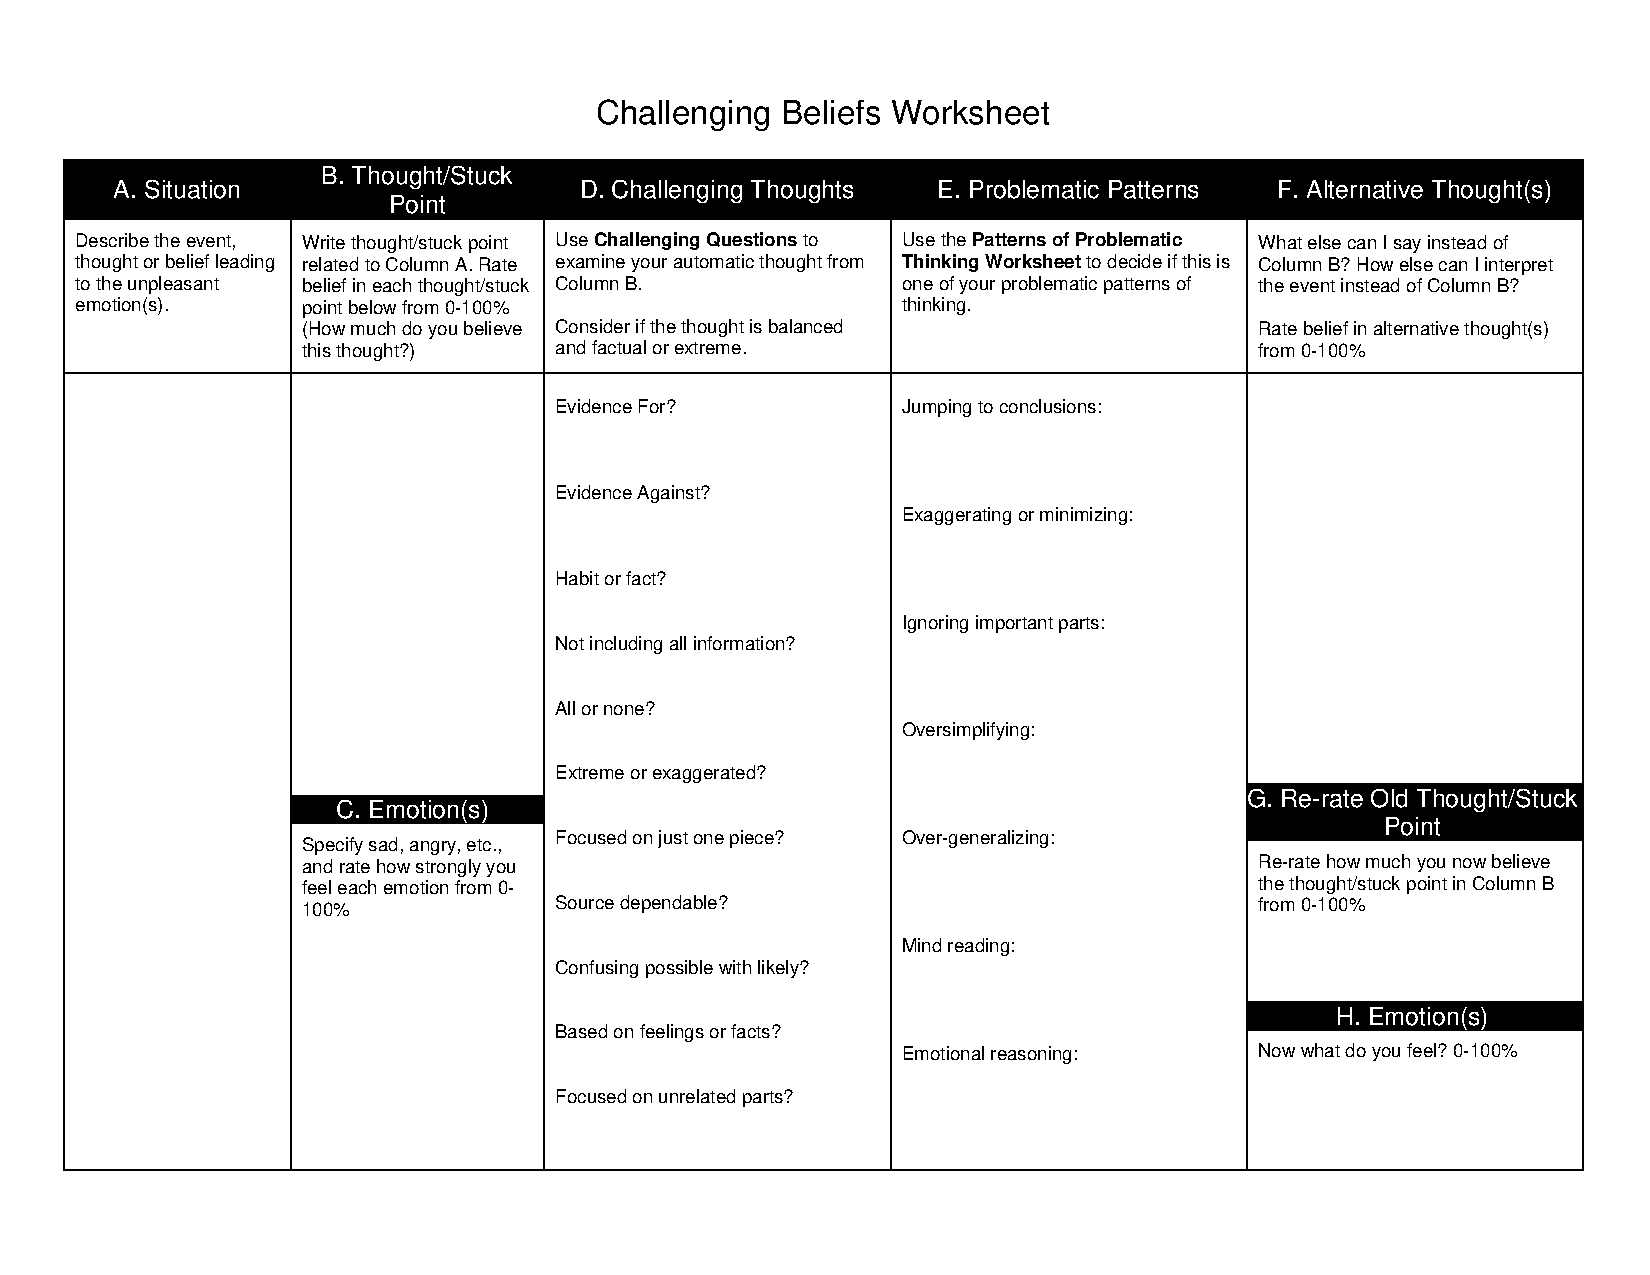
\includepdf[angle={270}]{challenging_beliefs.pdf}
\printbibliography
\label{sec:bibliography}
\addcontentsline{toc}{section}{\bibname}

\end{document}